\chapter{Geometria z algebrą liniową}

Materiały teoretyczne z geometrii z algebrą liniową zostały opracowane na podstawie \href{https://www.mimuw.edu.pl/~pbechler/inf_gal/}{skryptu Pawła Bechlera}, \href{https://www.ap.uj.edu.pl/diplomas/149716/?_s=1}{skryptu Lechosława Grochowskiego} oraz filmów \href{https://www.youtube.com/c/3blue1brown/}{3Blue1Brown}.

\section*{Podstawa programowa}
\begin{enumerate}
    \item Definicja \textbf{grupy} i grupy przemiennej.
    \item Ciała \textbf{liczb rzeczywistych} i \textbf{zespolonych}.
    \item \textbf{Przestrzenie liniowe}, liniowa niezależność wektorów, baza i wymiar przestrzeni liniowej.
    \item \textbf{Macierze i przekształcenia liniowe}, wyznaczniki.
    \item \textbf{Wektory i wartości własne} macierzy i przekształceń liniowych.
    \item Istnienie i jednoznaczność rozwiązań \textbf{układów liniowych}, eliminacja Gaussa.
    \item Przestrzenie z \textbf{iloczynem skalarnym}.
\end{enumerate}

\section{Grupy i ciała}

W zbiorze liczb rzeczywistych mamy zdefiniowane dwa działania jednoargumentowe:
\begin{itemize}
    \item wyznaczenie \textbf{liczby przeciwnej} do danej: $x\mapsto-x$,
    \item dla liczby różnej od zera, wyznaczenie jej \textbf{odwrotności}: $x\mapsto\frac{1}{x}=x^{-1}$.
\end{itemize}

Analogicznie, definiujemy także działania dwuargumentowe -- \textbf{dodawanie} oraz \textbf{mnożenie} dwóch liczb: $(x,y)\mapsto x+y$, $(x,y)\mapsto x\cdot y$. Odejmowanie i dzielenie można otrzymać jako złożenie odpowiednich operacji jedno- i dwuargumentowych.

Działania dodawania i mnożenia mają następujące własności:
\begin{itemize}
    \item Dla dowolnych $a,b\in\RR$ zachodzi $a+b=b+a$ oraz $a\cdot b=b\cdot a$. Mówimy, że działania są \textbf{przemienne}.
    \item Dla dowolnych $a,b,c\in\RR$ zachodzi $a+(b+c)=(a+b)+c$ oraz $a\cdot(b\cdot c)=(a\cdot b)\cdot c$. Mówimy, że działania są \textbf{łączne}.
    \item Dla dowolnych $a,b,c\in\RR$ zachodzi $a\cdot(b+c)=a\cdot b+a\cdot c$. Mówimy, że \textbf{mnożenie jest rozdzielne względem dodawania}.
\end{itemize}

W zbiorze liczb rzeczywistych istnieją również pewne szczególne elementy, które oznaczamy symbolami 0 i 1. Dla dowolnej liczby $a \in \RR$:
$$a + 0 = 0 + a = a \textqq{oraz} a \cdot 1 = 1 \cdot a = a$$

Liczby te nazywamy \textbf{elementem neutralnym} odpowiednio dodawania i mnożenia.
\bigskip

Nie zawsze prawdą jest, że wynik działania jedno- lub dwuargumentowego musi należeć do tego samego zbioru, co liczby wejściowe. Jeśli tak jest, to mówimy, że dany zbiór jest \textbf{zamknięty} ze względu na rozważane działanie lub że dane działanie jest działaniem \textbf{wewnętrznym} w tym zbiorze.

\begin{example}
    Oto kilka przykładów zamkniętości wybranych podzbiorów $\RR$ ze względu na podstawowe działania:
    \begin{itemize}
        \item W liczbach całkowitych $\ZZ$ wewnętrzne jest działanie wyznaczenia liczby przeciwnej, natomiast własności tej nie ma działanie wyznaczenia liczby odwrotnej.
        \item Zbiór liczb rzeczywistych różnych od zera $\RR_{\neq 0}$ jest zamknięty na działanie mnożenia, ale nie jest zamknięty na działanie dodawania (bo np. $1 + (-1) = 0 \notin \RR_{\neq 0}$).
    \end{itemize}
\end{example}

\subsection{Grupy}

Jeśli zbiór jest jednocześnie zamknięty ze względu na dane działanie dwuargumentowe (dodawanie lub mnożenie) i odpowiadające mu działanie jednoargumentowe (liczba przeciwna lub odwrotna), a dodatkowo element neutralny danego działania też należy do tego zbioru, to mówimy, że taki zbiór jest \textbf{grupą}. Formalna definicja jest następująca:

Zbiór $G$ wraz z
\begin{itemize}
    \item elementem wyróżnionym $e\in G$,
    \item działaniem dwuargumentowym ,,$\diamond$'' o własnościach
    \begin{itemize}
        \item zbiór $G$ jest zamknięty ze względu na ,,$\diamond$''
        \item dla dowolnych $x, y, z \in G$ zachodzi $x \diamond (y \diamond z) = (x \diamond y) \diamond z$ \gray{(łączność)}
        \item dla dowolnego $x \in G$ zachodzi $e \diamond x = x \diamond e = x$ \gray{(element neutralny)}
        \item dla każdego $x \in G$ istnieje $y \in G$, taki że $x \diamond y = e$ \gray{(element odwrotny)}
    \end{itemize}
\end{itemize}
nazywamy grupą z działaniem ,,$\diamond$'' i elementem neutralnym $e$. Grupę możemy zapisać jako trójkę uporządkowaną $(G,\diamond,e)$.

Jeżeli dodatkowo spełniony jest warunek przemienności (dla każdych $x, y \in G$ zachodzi $x \diamond y = y \diamond x$), to taką grupę nazywamy grupą \textbf{abelową} lub \textbf{przemienną}.

\begin{example}
    Oto kilka przykładów grup (oraz struktur, które grupami nie są):
    \begin{itemize}
        \item Zbiór $\ZZ$ z działaniem ,,$+$'' i elementem neutralnym 0 jest grupą abelową -- w oczywisty sposób spełnia on wszystkie warunki wymienione w definicji grupy.
        \item Zbiór $\RR$ z działaniem ,,$\cdot$'' i elementem neutralnym 1 nie jest grupą, ponieważ liczba 0 nie posiada elementu odwrotnego.
        \item Niech $\ZZ_n=\{0,1,\ldots,n-1\}$ oraz oznaczmy przez ,,$+$'' dodawanie modulo $n$. Wówczas $(\ZZ_n,+,0)$ jest $n$-elementową grupą abelową (dla dowolnego $n$).
    \end{itemize}
\end{example}

\subsection{Ciała}

Jak łatwo zauważyć, w zbiorze liczb rzeczywistych $\RR$ mamy do czynienia z dwiema podstawowymi grupami, jedną z dodawaniem, a drugą z mnożeniem:
$$(\RR, +, 0) \textqq{oraz} (\RR_{\neq 0}, \cdot, 1)$$

Taki opis struktury zbioru liczb rzeczywistych nie uwzględnia jednak tego, że działanie mnożenia jest rozdzielne względem dodawania. W związku z tym wprowadzamy jeszcze jedną strukturę: \textbf{ciało}.

Ciałem nazywamy zbiór $X$ wraz z działaniami ,,$+$'' i ,,$\cdot$'', zwanymi dodawaniem i mnożeniem, oraz wyróżnionymi elementami 0 i 1, taki że
\begin{itemize}
    \item $(X,+,0)$ jest grupą abelową,
    \item mnożenie jest przemienne i łączne oraz $(X\backslash\{0\},\cdot,1)$ jest grupą abelową,
    \item mnożenie jest rozdzielne względem dodawania.
\end{itemize}
Ciało możemy zapisać jako piątkę uporządkowaną $(X,+,\cdot,0,1)$.

\begin{example}
    Oto przykłady ciał:
    \begin{itemize}
        \item Ciało liczb rzeczywistych: $(\RR, +, \cdot, 0, 1)$.
        \item Ciało liczb wymiernych: $(\QQ, +, \cdot, 0, 1)$.
        \item Dla liczby pierwszej $p$ oraz ,,$+$'' i ,,$\cdot$'' jako dodawania i mnożenia modulo $p$, $(\ZZ_p,+,\cdot,0,1)$ jest ciałem mającym $p$ elementów (\textit{dla koneserów:} jest to przykład ciała Galois).
    \end{itemize}
\end{example}

\begin{problems}
    \prob Niech $(G, \diamond, e)$ będzie grupą, $a, b, c \in G$ i $a \diamond c = e$. Wtedy
    \answers{$a \diamond b = b \diamond a$}{$a \diamond c = c \diamond a$}{$(b \diamond a) \diamond (c \diamond b) = b \diamond b$}

    \prob Niech $\mathbb{G}=(G, \circ, e)$ będzie grupą. Rozważmy grupę $\mathbb{G}^{op}=(G, \cdot, e)$, gdzie $x \cdot y = y \circ x$ dla $x,y \in G$. Wtedy
    \answers{dla funkcji $f: \mathbb{G} \to \mathbb{G}$ określonej wzorem $f(x) = x^{-1}$ oraz dowolnej podgrupy $\mathbb{H}=(H,\circ,e)$ grupy $\mathbb{G}$ zbiór $f(\mathbb{H})$ jest podgrupą grupy $\mathbb{G}^{op}$}{grupy $\mathbb{G}$ i $\mathbb{G}^{op}$ są izomorficzne}{$\mathbb{G}=\mathbb{G}^{op}$ wtedy i tylko wtedy, gdy grupa $\mathbb{G}$ jest abelowa}
\end{problems}

\section{Liczby zespolone}

Oznaczmy obiekt $\sqrt{-1}$ jako $i$ (\textbf{jednostka urojona}). Co jasne, nie jest to liczba rzeczywista, ale taki obiekt okazuje się bardzo przydatny -- pozwala nam na spierwiastkowanie dowolnej liczby rzeczywistej ujemnej, np. $(5i)^2 = -25$ albo $(i\sqrt{2})^2 = -2$.

Takie obiekty postaci $bi$, gdzie $b \in \RR$ możemy dodać do znanych już liczb rzeczywistych, tworząc obiekty typu $a + bi$ (dla $a, b \in \RR$), czyli \textbf{liczby zespolone}. Zespolone z dwóch części: rzeczywistej (tej bez $i$) oraz urojonej (tej z $i$). Formalnie, jeśli $z=a+bi$, to
\begin{itemize}
    \item liczbę rzeczywistą $a$ nazywamy \textbf{częścią rzeczywistą} liczby zespolonej $z$ i oznaczamy $\purple{\Re z}$,
    \item liczbę rzeczywistą $b$ nazywamy \textbf{częścią urojoną} liczby zespolonej $z$ i oznaczamy $\purple{\Im z}$,
\end{itemize}

Zbiór wszystkich liczb zespolonych oznaczamy symbolem $\CC$ (ang. \textit{complex}). Na zbiorze $\CC$ mamy określone działania:
\begin{itemize}
    \item \textbf{dodawania}:
    $$
    (a+bi)+(c+di)=(a+c)+(b+d)i
    $$
    z elementem neutralnym $0=0+0i$,
    \item \textbf{mnożenia}:
    $$
    (a+bi)\cdot(c+di)=(ac-bd)+(ad+bc)i
    $$
    z elementem neutralnym $1=1+0i$,
    \item wyznaczenia \textbf{liczby przeciwnej} do $z=a+bi$:
    $$
    -z=-a-bi,
    $$
    takiej że $z+(-z)=0$,
    \item wyznaczenia \textbf{liczby odwrotnej} do $z=a+bi$:
    $$
    z^{-1}=\frac{1}{z}=\frac{1}{a+bi}=\frac{a}{a^2+b^2}-\frac{b}{a^2+b^2}i,
    $$
    takiej że $z\cdot z^{-1}=1$.
\end{itemize}

\textbf{Sprzężenie} liczby zespolonej $z = a + bi$ definiujemy jako
$$\overline{z}=a-bi$$

Jest to o tyle ciekawy obiekt, że pozwala nam na pokazanie ważnej własności wielomianów: \purple{jeśli wielomian zmiennej zespolonej o współczynnikach rzeczywistych ma pierwiastek nierzeczywisty, to ma również pierwiastek do niego sprzężony}. \; \textbf{\red{(przyp. red.: potrzebny przykład)}}

\subsection{Interpretacja wektorowa}

Skoro liczby zespolone, podobnie jak punkty na płaszczyźnie, możemy jednoznacznie definiować parami liczb rzeczywistych $(a, b) := a + bi$, to ich naturalną reprezentacją jest \textbf{płaszczyzna zespolona}, czyli układ współrzędnych, w którym osi $x$-ów odpowiada część rzeczywista, a osi $y$-ów -- część zespolona. W ten sposób możemy interpretować liczby zespolone jako wektory.

Zauważmy, że wtedy dodawanie liczb zespolonych jest jak dodawanie wektorów z $\RR^2$, co obrazuje poniższy rysunek:

\begin{center}
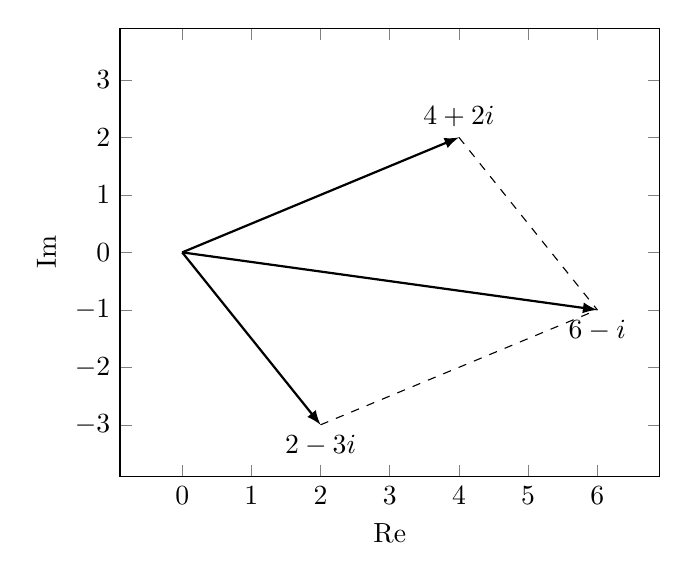
\begin{tikzpicture}
    \begin{axis}[
        xmin = -0.9, xmax = 6.9,
        ymin = -3.9, ymax = 3.9,
        xlabel = Re,
        ylabel = Im,
        xtick distance = 1,
        ytick distance = 1,
    ]
    \draw[thick, -latex] (axis cs: 0, 0) -- (axis cs: 4, 2) node[above] {$4 + 2i$};
    \draw[thick, -latex] (axis cs: 0, 0) -- (axis cs: 2, -3) node[below] {$2 - 3i$};
    \draw[thick, -latex] (axis cs: 0, 0) -- (axis cs: 6, -1) node[below] {$6 - i$};
    \draw[dashed] (axis cs: 4, 2) -- (axis cs: 6, -1);
    \draw[dashed] (axis cs: 2, -3) -- (axis cs: 6, -1);
    \end{axis}
\end{tikzpicture}
\end{center}

Podobnie jak dla liczb rzeczywistych, tak i dla zespolonych można zdefiniować \textbf{moduł} jako odległość od zera w układzie współrzędnych: dla $z = a + bi$ mamy
$$|z| = \sqrt{a^2 + b^2}$$

Dla tak określonego modułu zachodzi również \textbf{nierówność trójkąta}: dla dowolnych $z, w \in \CC$
$$|z + w| \leq |z| + |w|$$

\subsection{Postać trygonometryczna}

Do liczb zespolonych można wprowadzić koncepcję współrzędnych biegunowych -- zamiast określać wektor jako parę współrzędnych $x, y$, będziemy ustalać jego długość i kąt skierowania.

Niech $z=x+iy\in\CC$ i $z\neq0$. Oznaczmy literą $\phi$ kąt pomiędzy półosią rzeczywistą dodatnią i wektorem odpowiadającym $z$ i ustalmy, że jest to kąt zorientowany przeciwnie do ruchu wskazówek zegara. Wówczas $\cos\phi = \frac{x}{|z|}$, $\sin\phi = \frac{y}{|z|}$ oraz
$$
\purple{z = |z|(\cos\phi + i\sin\phi)}
$$
Kąt $\phi$ nazywamy \textbf{argumentem} liczby zespolonej $z$ i oznaczamy $\phi = \arg z$.

\begin{center}
\begin{tikzpicture}
    \begin{axis}[
        xmin = -0.9, xmax = 3.9,
        ymin = -0.9, ymax = 2.9,
        xlabel = Re,
        ylabel = Im,
        xtick = {3},
        ytick = {2},
        xticklabels = {$|z| \cos \phi$},
        yticklabels = {$i |z| \sin \phi$}
    ]
    \draw[thick, -latex] (axis cs: 0, 0) -- (axis cs: 3, 2) node[above] {$z$};
    \draw[dashed] (axis cs: 0, 2) -- (axis cs: 3, 2);
    \draw[dashed] (axis cs: 3, 0) -- (axis cs: 3, 2);
    \draw[-latex] (axis cs: 1, 0) arc [radius = 17mm, start angle = 0, end angle = 26]
        node[right, pos = 0.5] {$\phi$};
    \end{axis}
\end{tikzpicture}
\end{center}

Przy powyższym zapisie, mając $z = |z|(\cos\phi + i\sin\phi)$ i $w = |w|(\cos\theta + i\sin\theta)$, możemy zgrabnie wymnożyć obie liczby:
$$
zw = |z|\cdot|w|(\cos(\phi+\theta)+i\sin(\phi+\theta)).
$$

Widzimy więc, że przy mnożeniu liczb zespolonych ich moduły się mnożą, a argumenty dodają.

\begin{center}
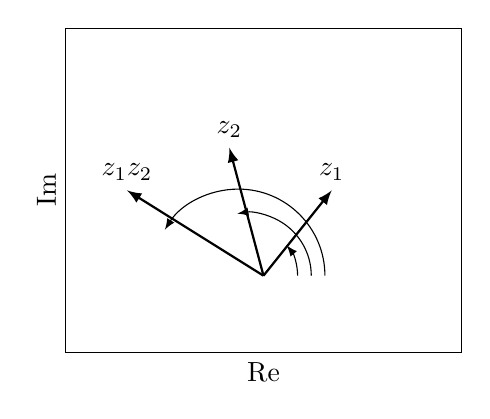
\begin{tikzpicture}
    \begin{axis}[
    	height = 5.7cm,
        xmin = -2.9, xmax = 2.9,
        ymin = -0.9, ymax = 2.9,
        xlabel = Re,
        ylabel = Im,
        xtick = \empty,
        ytick = \empty,
    ]
    \draw[thick, -latex] (axis cs: 0, 0) -- (axis cs: 1, 1) node[above] {$z_1$};
    \draw[-latex] (axis cs: 0.5, 0) arc [radius = 6mm, start angle = 0, end angle = 40];
    \draw[thick, -latex] (axis cs: 0, 0) -- (axis cs: -0.5, 1.5) node[above] {$z_2$};
    \draw[-latex] (axis cs: 0.7, 0) arc [radius = 8mm, start angle = 0, end angle = 100];
    \draw[thick, -latex] (axis cs: 0, 0) -- (axis cs: -2, 1) node[above] {$z_1z_2$};
    \draw[-latex] (axis cs: 0.9, 0) arc [radius = 11mm, start angle = 0, end angle = 148];
    \end{axis}
\end{tikzpicture}
\end{center}

Postać trygonometryczną możemy skrócić do \textbf{zapisu wykładniczego}:
$$
\purple{e^{i\phi} = \cos\phi+i\sin\phi}.
$$
Przy tym zapisie mnożenie liczb zespolonych wygląda prościej:
$$zw = |zw|e^{i(\phi+\theta)}$$

Potęgowanie liczb zespolonych możemy w łatwy sposób wykonać, wykorzystując \textbf{wzór de Moivre'a}:
jeżeli liczba $n$ jest całkowita, natomiast $z=|z|e^{i\phi}=|z|(\cos\phi + i\sin\phi)$, to
$$
\purple{z^n = |z|^ne^{in\phi} = |z|^n(\cos{n\phi} + i\sin{n\phi})}.
$$

\begin{example}
    Obliczymy $(1+i)^{21}$. W postaci trygonometrycznej mamy $1+i=\sqrt{2}(\cos\frac{\pi}{4}+i\sin\frac{\pi}{4})$, zatem
    $$
    (1+i)^{21} = (\sqrt{2})^{21}\left(\cos\frac{21\pi}{4}+i\sin\frac{21\pi}{4}\right) = 2^{10}\sqrt{2}\left(\cos\frac{5\pi}{4}+i\sin\frac{5\pi}{4}\right) = 2^{10}(-1-i)
    $$
\end{example}

\subsection{Pierwiastki zespolone}

Rozpatrzymy rozwiązania równania postaci $x^n = z$, gdzie $z \in \CC \backslash \{0\}$. Każde takie rozwiązanie $x \in \CC$ będziemy nazywać \textbf{pierwiastkiem zespolonym} stopnia $n$ z liczby zespolonej $z$.

Równanie $x^n = z$ ma zawsze $n$ pierwiastków, które są postaci
$$
x_k = \sqrt[n]{|z|} e^{i(\phi+2k\pi)/n} = \sqrt[n]{|z|}\left(\cos\left(\frac{\phi+2k\pi}{n}\right) + i\sin\left(\frac{\phi+2k\pi}{n}\right)\right).
$$

Zwróćmy uwagę, że pierwiastek zespolony to nie liczba, a zbiór liczb. Geometrycznie są one wierzchołkami wielokąta foremnego wpisanego w okrąg o środku w punkcie $(0, 0)$ i promieniu $\sqrt[n]{|z|}$ (dla $n = 2$ otrzymujemy dwa punkty symetryczne względem zera). Wyjaśnienie tego faktu jest intuicyjnie proste: o ile w liczbach rzeczywistych przyjmujemy jako pierwiastki zawsze wartości dodatnie, odrzucając ujemne (np. $\sqrt{9} = 3$, mimo że $(-3)^2$ to też 9), o tyle w liczbach zespolonych nie ma powodu, żeby wyróżniać którykolwiek z pierwiastków.

% TODO: rysunek

Rozpatrzymy jeszcze jeden szczególny przypadek: gdy $z = 1$, otrzymujemy następujący wzór na $n$ różnych zespolonych \textbf{pierwiastków z jedności} stopnia $n$:
$$
x_k = e^{i2k\pi/n} = \cos\left(\frac{2k\pi}{n}\right) + i\sin\left(\frac{2k\pi}{n}\right).
$$

Zauważmy, że wtedy $1 = 1 + 0i$ zawsze jest jednym z pierwiastków. Graficznie wystarczy więc wyznaczyć wierzchołki $n$-kąta foremnego położonego na okręgu o promieniu 1, którego jednym z wierzchołków jest jedynka.

% TODO: rysunek

\begin{editorsnote}
    Do sekcji ,,pierwiastki zespolone'' warto byłoby dodać rysunki.
\end{editorsnote}

\begin{problems}
    \prob Liczba zespolona $x_0$ jest rozwiązaniem równania $x^2 + x + 1 = 0$. Wynika z tego, że
    \answers{liczba $x_0^2$ też jest rozwiązaniem tego równania}{liczba $1/x_0$ też jest rozwiązaniem tego równania}{$x_0^3 = 1$}

    \prob Strukturę grupy z działaniem mnożenia liczb zespolonych i 1 jako elementem neutralnym ma zbiór
    \answers{$\{2^kz \in \CC \ : \; z^{2019} = 1\}$}{$\{z \in \CC \ : \; \Re(z) \cdot \Im(z) = 0\}$}{$\{z \in \CC \ : \ k \in \ZZ, \ |z| = 1\}$}
\end{problems}

\section{Przestrzenie liniowe}

Aby móc odpowiednio wprowadzić intuicję stojącą za przestrzeniami liniowymi, zaczniemy od ujednolicenia pojęcia \textbf{wektora}. Rozważając zagadnienia algebry liniowej umawiamy się, że \purple{punktem przyłożenia każdego z rozważanych wektorów jest zero} (o zadanym wymiarze, a więc może to być np. $(0, 0), (0, 0, 0)$ itd.).

Ponadto, w wielu przypadkach będziemy \purple{utożsamiać pojęcie punktu z pojęciem wektora}, tzn. punkt $(x, y)$ będziemy intuicyjnie kojarzyć z wektorem o początku w zerze i końcu w punkcie $(x, y)$. W związku z tym współrzędne wektora zapisujemy czasem w nawiasach okrągłych (jak w przypadku punktu) i nie zawsze używamy notacji nawiasów kwadratowych.

\begin{example}
	Punkt $(3, 2)$ można utożsamiać z wektorem $(3, 2)$, co pokazuje poniższy rysunek.
	
	\begin{center}
	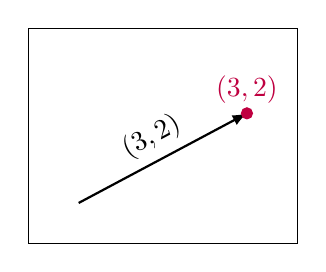
\begin{tikzpicture}
		\begin{axis}[
			width = 5cm,
			xmin = -0.9, xmax = 3.9,
			ymin = -0.9, ymax = 3.9,
			xtick = \empty,
			ytick = \empty,
			]
			\draw[thick, -latex] (axis cs: 0, 0) -- (axis cs: 3, 2)
				node[above, pos = 0.5, sloped] {$(3, 2)$};
                \draw[purple, fill] (axis cs: 3, 2) circle (2pt)
				node[above] {$(3, 2)$};
		\end{axis}
	\end{tikzpicture}
	\end{center}
\end{example}

Oznaczmy przez $\KK$ pewne ciało i przez $V$ zbiór pewnych wektorów, taki że $(V, +, 0)$ jest grupą abelową. Załóżmy też, że w zbiorze $X$ określone jest działanie ,,$\cdot$'' mnożenia wektora $\vec{v} \in V$ przez skalar $a \in \KK$, przy czym spełnia ono następujące własności: dla dowolnych $a, b \in \KK$ i $\vec{v}, \vec{w} \in V$
\begin{itemize}
	\item mnożenie przez skalar jest rozdzielne względem dodawania wektorów:
	$$a(\vec{v} + \vec{w}) = a\vec{v} + a\vec{w},$$
	
	\item mnożenie przez wektor jest rozdzielne względem dodawania skalarów:
	$$(a + b)\vec{v} = a\vec{v} + b\vec{v},$$
	
	\item dwukrotne mnożenie wektora przez skalar można zastąpić mnożeniem skalarów:
	$$a \cdot (b \cdot \vec{v}) = (a \cdot b) \cdot \vec{v},$$
	
	\item elementem neutralnym mnożenia przez skalar jest element neutralny mnożenia skalarów $1 \in \KK$:
	$$1 \cdot \vec{v} = \vec{v}.$$
\end{itemize}

Wówczas zbiór $V$ wraz z tak zdefiniowanymi działaniami ,,$+$'' i ,,$\cdot$'' jest \textbf{przestrzenią liniową} nad ciałem $\KK$. Elementy przestrzeni liniowej nazywamy wektorami, a ciała $\KK$ -- skalarami.

\begin{example}
	Oto kilka przykładów przestrzeni liniowych (oraz struktur, które przestrzeniami liniowymi nie są):
	
	\begin{itemize}
		\item Standardowa przestrzeń rzeczywistych wektorów $n$-wymiarowych $\RR^n$ jest, w oczywisty sposób, przestrzenią liniową nad $\RR$. Nie jest ona jednak przestrzenią liniową nad $\CC$, gdyż np. mamy $i \cdot (1, 1) = (i, i)$ -- pomnożenie wektora z $\RR^n$ przez skalar z $\CC$ sprawia, że opuszczamy przestrzeń wektorów rzeczywistych.
		
		\item Ogół funkcji wielomianowych jednej zmiennej rzeczywistej $x$ o współczynnikach rzeczywistych $\RR[x]$ jest przestrzenią liniową nad $\RR$. Przykładowo, $x^2 + 1$ oraz $2x^3 + 5x^2 + 3$ są wektorami tej przestrzeni. Możemy je do siebie dodawać i mnożyć przez rzeczywiste skalary, a działania te spełniają wszystkie warunki wymagane w definicji przestrzeni liniowej.
		
		\item Wektory z $\RR^2$ postaci $\{(2a, a) \ | \ a \in \RR\}$ rozpinają przestrzeń liniową. Gdybyśmy narysowali zbiór punktów tożsamych z tymi wektorami, uzyskalibyśmy prostą przechodzącą przez $(0, 0)$. Nie jest jednak prawdą, że punkty z dowolnej prostej utworzą przestrzeń wektorową. Na przykład, punkty z prostej o równaniu $y = x + 1$ są postaci $(x, x + 1)$ i nie tworzą przestrzeni wektorowej, gdyż m.in. punkty $(0, 1)$ i $(1, 2)$ do niej należą, a ich suma $(1, 3)$ -- już nie.
	\end{itemize}
\end{example}

Jak widać, wektorami mogą być obiekty dość dalekie od definicji ze szkoły średniej (czyli przestrzeni $\RR^n$). Takie ogólne podejście pozwoli przenosić wiele ciekawych zależności ze standardowego $\RR^n$ do innych struktur.
\bigskip

Fakt istnienia w przestrzeniach liniowych \textbf{wektora i skalara zerowego} definiuje nam kilka dodatkowych własności: jeżeli $V$ jest przestrzenią liniową nad ciałem $\KK$, to dla każdego wektora $\vec{v} \in V$ oraz skalara $a \in \KK$ zachodzą zależności:
\begin{itemize}
    \item $0 \cdot \vec{v} = a \cdot \vec{0} = 0$ (gdzie ,,$0$'' po lewej to zero w ciele $\KK$, a ,,$\vec{0}$'' po prawej to element neutralny dodawania w $V$),
    \item $a\vec{v} = \vec{0} \wtw a = 0 \ \lor \ \vec{v} = \vec{0}$,
    \item $(-a)\vec{v} = a(-\vec{v}) = -(a\vec{v})$, gdzie przez $-\vec{v} \in V$ rozumiemy wektor przeciwny do $\vec{v}$.
\end{itemize}

\subsection{Podprzestrzenie liniowe}

Załóżmy, że $V$ jest przestrzenią liniową nad ciałem $\KK$ i $P \subset V$ jest jej niepustym podzbiorem, który, wraz z odziedziczonymi z $V$ działaniami dodawania i mnożenia przez skalar, także jest przestrzenią liniową nad $\KK$. Mówimy wówczas, że $P$ jest \textbf{podprzestrzenią liniową} przestrzeni $V$.

\begin{example}
	Weźmy przestrzeń $\RR^2$ nad $\RR$. Jej przykładową podprzestrzenią jest zbiór $\{(3a, 5a) \ | \ a \in \RR\}$. Z kolei przykładową podprzestrzenią tej przestrzeni jest $\{\vec{0}\}$ -- podprzestrzeń jednoelementowa, składająca się wyłącznie z wektora zerowego.
\end{example}

Prawdą jest, że $P \neq \pusty$ jest podprzestrzenią liniową $V$ wtedy i tylko wtedy, gdy zachodzą wszystkie z poniższych warunków:
\begin{itemize}
	\item $\vec{0} \in P$
    \item dla dowolnych $\vec{v}, \vec{w} \in P$ także $\vec{v} + \vec{w} \in P$,
    \item dla dowolnych $\vec{v} \in P$ i $a \in \KK$ także $a \vec{v} \in P$.
\end{itemize}

\subsection{Liniowa niezależność}

Załóżmy, że $V$ jest przestrzenią liniową nad ciałem $\KK$. \textbf{Kombinacją liniową wektorów} $\vec{v_1}, ..., \vec{v_n} \in V$ o współczynnikach $a_1, ..., a_n \in \KK$ nazywamy każdy z wektorów postaci
$$\vec{v} = a_1\vec{v_1} + ... + a_n\vec{v_n}.$$

\begin{example}
    Każdy wektor $\vec{v} \in \RR^3$ jest kombinacją liniową wektorów jednostkowych $\vec{e_1} = (1, 0, 0), \vec{e_2} = (0, 1, 0), \vec{e_3} = (0, 0, 1)$:
    $$\vec{v} = (a_1, a_2, a_3) = a_1\vec{e_1} + a_2\vec{e_2} + a_3\vec{e_3}$$
\end{example}

Niech $V$ będzie przestrzenią liniową, natomiast $G \subset V$ pewnym zbiorem wektorów. Najmniejszą podprzestrzeń liniową zawierającą wszystkie wektory z $G$ nazywamy \textbf{podprzestrzenią rozpiętą} przez $G$ i oznaczamy jako
$\purple{\spn{G}}$. Jeżeli $G = \{\vec{g_1}, ..., \vec{g_k}\}$, to
$$\purple{\spn{G} = \{a_1\vec{g_1} + ... + a_k\vec{g_k} \ | \ a_1, ..., a_k \in \KK\}}$$

Podprzestrzenie rozpięte przez pewien zbiór wektorów składają się więc ze wszystkich kombinacji liniowych wektorów z tego zbioru.

\begin{example}
    Weźmy przestrzeń funkcji wielomianowych $\RR[x]$. Wtedy $\spn{\{1, x^2\}}$ to ogół wielomianów postaci $w(x) = ax^2 + b$, gdzie $a, b \in \RR$. Z kolei $\spn{\{1, x^2 + 1\}}$ to ogół wielomianów postaci $w(x) = c(x^2 + 1) + d$, gdzie $c, d \in \RR$, czyli tak naprawdę ogół wielomianów postaci $w(x) = ax^2 + b$ -- taka zmiana zbioru rozpinającego przestrzeń nie dała w tym wypadku niczego nowego.
    
    A czym jest $\spn{\{x^2 + 1\}}$? To zbiór wszystkich wielomanów postaci $ax^2 + a$ dla $a \in \RR$. Jest on mniejszy niż poprzedni (tzn. poprzedni ma wszystkie występujące tu wielomiany i jeszcze jakieś inne, np. $x^2 + 2$).
\end{example}

\begin{example}
	Pozostańmy w przestrzeni $\RR[x]$. Tym razem weźmy jednak nieskończony zbiór rozpinający przestrzeń: $G = \{1, x, x^2, x^3, ...\}$. Widać, że w $\spn{G}$ znajdą się wszystkie wielomiany, a ponieważ wielomiany są podprzestrzenią, w $\spn{G}$ nie będzie nic więcej. Może trochę dziwić fakt, że choć np. $2x^3 + 5x^2 - 7x + 4 \in \spn{G}$, to $1 + x + x^2 + x^3 + ... \notin \spn{G}$ -- weźmy jednak pod uwagę, że w podprzestrzeniach rozpiętych mamy jedynie skończone sumy przeskalowanych wektorów bazowych.
\end{example}

\begin{example}
	Rozważmy przestrzeń $\RR^3$ i weźmy zbiór jednoelementowy $\{(1, 2, 3)\}$. Wtedy $$\spn{\{(1, 2, 3)\}} = \{a(1, 2, 3) \ | \ a \in \RR\},$$ czyli podprzestrzenią rozpiętą jest zbiór wszystkich przeskalowań wektora $(1, 2, 3)$, a więc wektory $$(0, 0, 0), (1, 2, 3), (2, 4, 6), (0.5, 1, 1.5), (-1, -2, -3) \ \text{itd.}$$ Geometrycznie będzie to prosta w $\RR^3$ przechodząca przez punkt $(0, 0, 0)$.
	
	Dodajmy teraz wektor $(2, 0, 3)$, otrzymując $$\spn{\{(1, 2, 3), (2, 0, 3)\}} = \{a(1, 2, 3) + b(2, 0, 3) \ | \ a, b \in \RR\}.$$ Ustalając $b = 0$ i wstawiając wszystkie możliwe $a$, wygenerujemy tę samą prostą, co poprzednio. Dla innych wartości $b$ otrzymamy inne proste, równoległe do siebie wzajemnie. Wszystkie te proste biegną w tym samym kierunku co wektor $(2, 0, 3)$, więc łącząc je wszystkie w całość dochodzimy do wniosku, że nasza przestrzeń $\spn{\{(1, 2, 3), (2, 0, 3)\}}$ to pewna płaszczyzna umieszczona w $\RR^3$ (złożona ze wszystkich powstałych prostych).
	
	A co ze $\spn{\{(1, 2, 3), (2, 0, 3), (-1, 2, -2)\}}$? Dodanie wektora $(-1, 2, -2)$ nie zmieni naszej przestrzeni -- wystarczy zauważyć, że $$(-1, 2, -2) = (1, 2, 1) + (-1)(2, 0, 3),$$ więc z pomocą $(-1, 2, -2)$ nie wygenerujemy żadnych nowych kombinacji liniowych.
\end{example}

Rozważając powyższe przykłady, zajmiemy się teraz kwestią zbędnych generatorów, czyli takich wektorów, których dodanie do zbioru rozpinającego przestrzeń nie ma żadnego wpływu na otrzymaną przestrzeń. Nietrudno zauważyć, że jeśli pewien wektor jest kombinacją liniową pozostałych wektorów, to można go odrzucić, gdyż nic nowego nie wniesie.

Zbiór wektorów nazywamy zbiorem wektorów \textbf{liniowo zależnych}, jeśli pewien element tego zbioru można przedstawić jako kombinacją liniową pewnych pozostałych.

Natomiast układ wektorów niespełniający powyższego warunku jest \textbf{liniowo niezależny}. Formalnie, ma on więc następującą własność: dla dowolnych $a_1, ..., a_n \in \KK$ zachodzi
$$a_1\vec{v_1} + ... + a_n\vec{v_n} = 0 \ \Leftarrow \ a_1 = ... = a_n = 0$$

\begin{example}
	Liniowo niezależny jest zbiór wektorów $\{(1, 0, 0), (1, 1, 0), (1, 1, 1)\}$ -- nie da się otrzymać żadnego z wektorów poprzez kombinację liniową pozostałych.
	
	Natomiast zbiór
	$$\{(1, 0, 0), (1, 1, 0), (1, 1, 1), (5, 6, 7)\}$$
	jest liniowo zależny, bo na przykład
	$$(5, 6, 7) = 7 \cdot (1, 1, 1) - (1, 1, 0) - (1, 0, 0)$$
\end{example}

Intuicyjnie, o liniowej niezależności możemy myśleć w następujący sposób: każdy wektor w zbiorze liniowo niezależnym niesie ze sobą \textit{pewną unikalną informację}, której nie da się uzyskać za pomocą pozostałych wektorów w tym zbiorze.

Przytoczymy jeszcze jeden ważny fakt: \purple{dowolny podzbiór zbioru wektorów liniowo niezależnych także jest liniowo niezależny}.

\subsection{Baza i wymiar przestrzeni liniowej}

Jeszcze raz przyjrzymy się kwestii zbędnych generatorów przestrzeni rozpiętych. Wiemy już, że kluczowa jest tu cecha liniowej niezależności zbioru rozpinającego przestrzeń.

Układ wektorów $\vec{v_1}, ..., \vec{v_n} \in V$ nazywamy \textbf{bazą} przestrzeni $V$, jeżeli jest on liniowo niezależny i rozpina przestrzeń $V$ (tj. $V = \spn{\{\vec{v_1}, ..., \vec{v_n}\}}$).

Co ważne, każdy wektor z przestrzeni \purple{zapisuje się dokładnie na jeden sposób} jako kombinacja liniowa wektorów z bazy tej przestrzeni. Intuicyjnie więc baza stanowi zbiór wektorów, z których ,,budujemy'' całą przestrzeń bazową (tj. wszystkie jej elementy).

Baza jest zarówno maksymalnym układem wektorów liniowo niezależnych w swojej przestrzeni, jak i minimalnym zbiorem wektorów rozpinających daną przestrzeń. Jak należy to rozumieć?
\begin{itemize}
	\item \purple{Każdy właściwy podzbiór bazy jest zbiorem liniowo niezależnym, rozpinającym pewną podprzestrzeń bazowej przestrzeni.} Intuicyjnie: skoro baza składa się z wektorów liniowo niezależnych, to usunięcie z niej dowolnego elementu zabiera nam \textit{pewną unikalną informację}, którą ten element wnosił. Co za tym idzie -- nie będziemy w stanie wygenerować (za pomocą kombinacji liniowych pozostałych elementów) niektórych elementów z bazowej przestrzeni, do których otrzymania był niezbędny usunięty przez nas element. Taki podzbiór bazy rozepnie więc pewną, mniejszą podprzestrzeń bazowej przestrzeni.
	
	\item \purple{Każdy właściwy nadzbiór bazy jest zbiorem liniowo zależnym.} Skoro baza rozpina całą przestrzeń, tj. nie ma w niej elementów, których nie dałoby się uzyskać poprzez kombinację liniową wektorów z bazy, to dodanie jakiegokolwiek elementu nie może przynieść nam już żadnej dodatkowej informacji, która pozwoliłaby nam uzyskać nowe elementy (bo takie nie istnieją). Mamy więc pewność, że każdy dodany do bazy element jest kombinacją liniową wektorów z bazy.
\end{itemize}

\begin{example}
    Rozważmy przestrzeń $\RR^3$ i jej \textbf{bazę kanoniczną} (tzn. złożoną z wektorów jednostkowych):
    $$\{(1, 0, 0), (0, 1, 0), (0, 0, 1)\}$$
   	Nietrudno sprawdzić, że rzeczywiście jest to baza: jej wektory są w oczywisty sposób liniowo niezależne, a każdy wektor z $\RR^3$ można zapisać jako liniową kombinację wektorów bazowych:
   	$$(a, b, c) = a(1, 0, 0) + b(0, 1, 0) + c(0, 0, 1)$$
   	
   	Inną przykładową bazą przestrzeni $\RR^3$ jest
   	$$\{(1, 0, 0), (7, 7, 0), (42, 42, 42)\}.$$
\end{example}

Z przedstawionych powyżej dwóch faktów możemy wywnioskować, że wszystkie bazy danej przestrzeni składają się z tej samej liczby wektorów. Tę liczbę nazywamy \textbf{wymiarem} przestrzeni liniowej $V$ i oznaczamy przez $\purple{\dim V}$. Jeżeli $V$ nie ma bazy skończonej, przyjmujemy $\dim V = \infty$.

\begin{example}
    Oto kilka przykładów wymiarów baz różnych przestrzeni:
    \begin{itemize}
    	\item Każda z przestrzeni $\RR^n$ dla $n \in \NN_+$ ma wymiar $n$, gdyż np. jej baza kanoniczna liczy właśnie $n$ elementów ($n$ wektorów bazowych, po jednym na każdą z $n$ współrzędnych wektora).
    	
    	\item Podprzestrzeń zerowa $\{(0, 0, 0)\}$ przestrzeni $\RR^3$ ma wymiar równy 0.
    	
    	\item Przestrzeń funkcji wielomianowych zmiennej rzeczywistej stopnia co najwyżej 2 o współczynnikach rzeczywistych ma wymiar 3, gdyż jej baza kanoniczna $\{1, x, x^2\}$ liczy właśnie 3 elementy.
    	
    	\item Przestrzeń $\RR[x]$ ma wymiar równy $\infty$ -- skończona baza nie pozwoliłaby bowiem zapisywać wielomianów odpowiednio wysokich stopni.
    \end{itemize}
\end{example}

Z pojęciem wymiaru związane są bardzo ważne własności.

Załóżmy, że $\dim{V} < \infty$ i $U \subseteq V$ jest podprzestrzenią liniową $V$. Wówczas
\begin{itemize}
	\item $\dim{U} \leq \dim{V}$,
	\item $\dim{U} = \dim{V}$ wtedy i tylko wtedy, gdy $U = V$.
\end{itemize}

Załóżmy, że $\dim{X}=n<\infty$. Wówczas
\begin{itemize}
    \item każdy liniowo niezależny układ wektorów z $X$ można uzupełnić do bazy przestrzeni $X$,
    \item z każdego układu wektorów rozpinających przestrzeń $X$ można wybrać bazę przestrzeni $X$,
    \item jeżeli pewne $n$ wektorów $x_1,\ldots,x_n\in X$ jest liniowo niezależne, to są one bazą przestrzeni $X$,
    \item jeżeli pewne $n$ wektorów $x_1,\ldots,x_n\in X$ rozpina przestrzeń $X$, to są one jej bazą.
\end{itemize}

\subsection{Przecięcie i suma podprzestrzeni}

Załóżmy, że $X$ jest przestrzenią liniową nad ciałem $\KK$ i $Y_j\subset X$ są podprzestrzeniami liniowymi, gdzie $j\in J$. Wówczas zbiór będący \textbf{przecięciem} tych przestrzeni,
$$
Y = \bigcap_{j\in J}Y_j,
$$
też jest podprzestrzenią liniową w $X$.

\begin{example}
    Przecięciem podprzestrzeni $U = \{ x \in \RR^3 : x_1 + x_2 = 0\}, V = \{x \in \RR^3 : x_2 + x_3 = 0\}$ jest
    $$U \cap V = \spn\big\{(1, -1, 1)\big\} \subset \RR^3$$
\end{example}

Załóżmy, że $X$ jest przestrzenią liniową nad ciałem $\KK$ i $U,V\subset X$ są podprzestrzeniami liniowymi. \textbf{Suma} podprzestrzeni $U$ i $V$ to zbiór
$$
U + V = \{u+v\in X : u\in U, v\in V\}.
$$
Taka suma podprzestrzeni też jest podprzestrzenią liniową w $X$.

W ogólności nie jest prawdą, że $U+V=U\cup V$. Łatwo widać, że $U\cup V\subset U+V$. Ponadto, zbiór $U\cup V$ nie musi być podprzestrzenią liniową w $X$.

Następujące warunki są równoważne:
\begin{itemize}
    \item $U\cap V=\{0\}$,
    \item dla każdego wektora $x\in U+V$ wektory $u\in U$ i $v\in V$ takie, że $x=u+v$ są wyznaczone jednoznacznie.
\end{itemize}

\begin{example}
    W przestrzeni wielomianów 3 stopnia o współczynnikach rzeczywistych $\RR[x]_3$ zachodzi
    $$\spn(1, x^2) + \spn(1 + x, x^2 + x^3) = \spn(1, x, x^2, x^3) = \RR[x]_3$$
\end{example}

Załóżmy, że $X$ jest przestrzenią liniową nad ciałem $\KK$ i $U,V\subset X$ są podprzestrzeniami liniowymi. Jeśli $U$ i~$V$ są rozłączne (tj. $U\cap V=\{0\}$), mówimy, że podprzestrzeń $U+V$ jest \textbf{sumą prostą} podprzestrzeni $U$ i~$V$ i~piszemy $U+V=\purple{U\oplus V}$.

\begin{example}
    W przestrzeni wielomianów 3 stopnia o współczynnikach rzeczywistych $\RR[x]_3$ zachodzi
    $$\spn(1, x^2) \oplus \spn(x, x^3) = \spn(1, x, x^2, x^3) = \RR[x]_3$$
\end{example}

Jeżeli $Y,Z\subset X$ są podprzestrzeniami skończonego wymiaru, to
\begin{itemize}
    \item wymiary podprzestrzeni $Y\cap Z$ oraz $Y+Z$ też są skończone,
    \item $\purple{\dim(Y+Z)=\dim{Y}+\dim{Z}-\dim(Y\cap Z)}$.
\end{itemize}

\begin{problems}
    \prob Niech $X$ będzie przestrzenią liniową wymiaru 15. Wynika z tego, że
    \answers{każdy układ 20 wektorów z $X$ jest liniowo zależny}{każdy układ 10 wektorów z $X$ jest liniowo niezależny}{każda baza $X$ składa się z 15 wektorów}

    \prob Dana jest przestrzeń $X$ wymiaru 10 oraz podprzestrzenie $U$, $V$, takie że $\dim(U) = \dim(V)$ oraz $X = U + V$. Wynika z tego, że
    \answers
    {$\dim(U) = 5$}
    {$\dim(U) \geq 5$}
    {$\dim(U \cap V) = 0$}
    
    \prob Dane są elementy przestrzeni liniowej nad ciałem liczb rzeczywistych $\Vec{a}, \Vec{b}, \Vec{c}$. Prawdą jest, że
    \answers{jeżeli $(\Vec{a}, \Vec{b}, \Vec{c})$ jest niezależny liniowo, to $(\Vec{a} - \Vec{b}, \Vec{b} - \Vec{c}, \Vec{c} - \Vec{a})$ jest niezależny liniowo}{jeżeli $(\Vec{a}, \Vec{b}, \Vec{c})$ jest niezależny liniowo, to $(\Vec{a} + \Vec{b}, \Vec{b} + \Vec{c}, \Vec{c} + \Vec{a})$ jest niezależny liniowo}{jeżeli $(\Vec{a} + \Vec{b}, \Vec{b} + \Vec{c}, \Vec{c} + \Vec{a})$ jest niezależny liniowo, to $(\Vec{a}, \Vec{b}, \Vec{c})$ jest niezależny liniowo}
\end{problems}

\section{Macierze i przekształcenia liniowe}

\textbf{Macierzą} (nad ciałem $\KK$) wymiaru $m \times n$ nazywamy tablicę prostokątną 
$$
\begin{bmatrix}
    a_{1,1} & a_{1,2} & \cdots & a_{1,n} \\
    a_{2,1} & a_{2,2} & \dots & a_{2,n} \\
    \vdots & \vdots & \ddots & \vdots \\
    a_{m,1} & a_{m,2} & \cdots & a_{m,n}     
\end{bmatrix}
$$
gdzie $a_{i,j} \in \KK$ dla $1 \leq i \leq m, \ 1 \leq j \leq n$. Można też zapisać taką macierz jako $$
A=[a_{i,j}]_{i=1,\dots,m, \ j=1,\dots,n}
$$
Macierz $m\times n$ ma $m$ wierszy i $n$ kolumn. \purple{Pierwszy indeks odpowiada wierszowi, a drugi kolumnie}. Piszemy wtedy, że macierz należy do zbioru macierzy $\KK^{m, n}$.

Specyficznym przypadkiem macierzy jest macierz $\KK^{n, 1}$ lub po prostu macierz $\KK^n$, którą nazywamy \textbf{wektorem} długości $n$:
$$
\vec{x} = \begin{bmatrix}
    x_1 \\ x_2 \\ \dots \\ x_n
\end{bmatrix}
$$

Przykłady innych często spotykanych macierzy:
\begin{itemize}
    \item \textbf{macierz zerowa} -- jej elementy to same zera,
    \item \textbf{macierz diagonalna} -- macierz kwadratowa zawierająca niezerowe wartości jedynie na diagonali (przekątnej), zapisujemy $D=\text{diag}(d_1,\dots, d_n)$,
    \item \textbf{macierz jednostkowa} rozmiaru $n \times x$, taka że $I_n=\text{diag}(1, \dots, 1)$,
    \item \textbf{macierz górno- i dolnotrójkątna} -- zawierająca niezerowe wartości jedynie na diagonali oraz ponad/poniżej niej,
    \item \textbf{macierz permutacji} -- macierz kwadratowa, która ma w każdym wierszu i w każdej kolumnie dokładnie jedną jedynkę oraz zera na pozostałych miejscach.
\end{itemize}

\subsection{Działania na macierzach}
Niech 
$$
A=\begin{bmatrix}
    a_{1,1} & a_{1,2} & \cdots & a_{1,n} \\
    a_{2,1} & a_{2,2} & \cdots & a_{2,n} \\
    \vdots & \vdots & \ddots & \vdots \\
    a_{m,1} & a_{m,2} & \cdots & a_{m,n}    
\end{bmatrix} \ \in \KK^{m,n}
$$
\textbf{Transpozycją macierzy} $A\in\KK^{m,n}$ nazywamy macierz
$$
A^T=\begin{bmatrix}
    a_{1,1} & a_{2,1} & \cdots & a_{m,1} \\
    a_{1,2} & a_{2,2} & \cdots & a_{m,2} \\
    \vdots & \vdots & \ddots & \vdots \\
    a_{1,n} & a_{2,n} & \cdots & a_{m,n}    
\end{bmatrix} \ \in \KK^{n,m}
$$
o zamienionych kolumnach z wierszami (dla macierzy niekwadratowych zmieniają się także wymiary macierzy). Macierz $A$ jest \textbf{symetryczna} jeśli zachodzi $A=A^T$ oraz \textbf{antysymetryczna} jeśli $A=-A^T$.

\textbf{Hermitowskie sprzężenie} macierzy $A$ to jej transpozycja wraz ze sprzężeniem każdego z jej elementów, na przykład
$$
\begin{bmatrix}
    1+i & 2 & 2 - i \\
    2 + 3i  & i & 0 \\
\end{bmatrix}^H = 
\begin{bmatrix}
    1 - i & 2 - 3i \\
    2 & -i \\
    2 + i & 0
\end{bmatrix}
$$
i, jak widać, $A^H=\overline{A^T}=(\overline{A})^T$. Macierz $A$ jest hermitowska, gdy $A=A^H$.

\textbf{Dodawanie i odejmowanie macierzy} określone jest \purple{jedynie dla macierzy o tych samych wymiarach} -- odpowiadające sobie elementy (o tych samych indeksach) należy dodać lub odjąć i utworzyć w ten sposób macierz wynikową.

\textbf{Mnożenie macierzy} $A$ z macierzą $B$ jest zdefiniowane jedynie, gdy \purple{$A$ jest wymiarów $m\times k$ oraz $B$ jest wymiarów $k \times n$}, czyli macierz po lewej musi mieć tyle kolumn, ile ta po prawej ma wierszy. Widać to, gdy zapiszemy macierze w sposób wygodny do mnożenia:

$$
\hspace{6em} \begin{bmatrix}
    1 & -1 & 1 & 2 \\
    2 & 0 & 1 & 3 \\
    3 & 1 & 1 & 4
\end{bmatrix}
$$
$$
\begin{bmatrix}
    1 & -1 & 2 \\
    0 & 3 & -2
\end{bmatrix}\cdot = 
\begin{bmatrix}
    5 & 1 & 2 & 13 \\
    0 & -2 & 1 & -17
\end{bmatrix}
$$

Własności mnożenia macierzy ($A, B, C$ są macierzami takimi, że odpowiednie działania są zdefiniowane, $c$~jest skalarem):
\begin{itemize}
    \item $(A + B)\cdot C = A\cdot C + B \cdot C$
    \item $A\cdot(B+C)=A\cdot B + A\cdot C$
    \item $c(A\cdot B) = cA \cdot B = A \cdot cB$
    \item $(A\cdot B)\cdot C = A\cdot(B\cdot C)$
    \item $(A\cdot B)^T = B^T\cdot A^T$
    \item jeśli $A$ to macierz zerowa, to $A\cdot B$ też jest zerowa
    \item $A\cdot B$ niekoniecznie wynosi $B\cdot A$, dla macierzy niekwadratowych nie jest w ogóle określone
    \item jeśli $A\cdot B = [0]_{m,n}$, to niekoniecznie $A$ lub $B$ muszą być macierzami zerowymi
\end{itemize}

Macierz kwadratowa $A \in \KK^{n,n}$ jest \textbf{nieosobliwa} (odwracalna), gdy istnieje macierz kwadratowa $A^{-1} \in \KK^{n,n}$ \textit{odwrotna} do niej, taka że $A \cdot A^{-1} = A^{-1} \cdot A = I_n$. Tylko dla macierzy kwadratowych istnieją macierze odwrotne.

\subsection{Wyznacznik macierzy}
Oznaczmy jako $A_{i,j} \in \KK^{n-1, n-1}$ macierz otrzymaną z macierzy $A \in \KK^{n, n}$ poprzez usunięcie $i$-tego wiersza i~$j$-tej kolumny. Niech $n=1,2,3,\dots$ oraz $A=[a_{i,j}]_{i,j=1}^n\in\KK^{n,n}$. \textbf{Wyznacznik} stopnia $n$ to funkcja \purple{$\det = \det_n:\KK^{n,n}\to \KK$} zdefiniowana w następujący sposób:
\begin{itemize}
    \item dla $n=1$: $\det_1[a_{1,1}]=a_{1,1}$,
    \item dla $n>1$: $\det_nA=\sum_{i=1}^n(-1)^{i+1}a_{i,1}\cdot \det_{n-1}A_{i,1}$ -- rozwinięcie Laplace'a.
\end{itemize}

\begin{example}
    Obliczymy wyznacznik macierzy o wymiarach $2 \times 2$ za pomocą rozwinięcia Laplace'a: jeśli $A = \begin{bmatrix}
        a & b \\ c & d
    \end{bmatrix}$, to
    $$\det A = \det_2 A = a \cdot \det_1 \Vect{d} - c \cdot \det_1 \Vect{b} = ad - bc$$
\end{example}

Przy liczeniu wyznaczników przydaje się także \textbf{twierdzenie Cauchy'ego}: jeżeli $A,B\in \KK^{n,n}$, to 
$$
\purple{\det_n(AB)=\det_n(A)\cdot \det_n(B)}.
$$

Rozważymy teraz \textbf{interpretację geometryczną wyznacznika}: odpowiada ona temu, jak macierz jako przekształcenie liniowe (o tym więcej w następnym dziale) \purple{skaluje pole powierzchni} przypadające na dany jej fragment:
\begin{figure}[H]
    \centering
    \includegraphics[scale=0.2]{rozdziały/images/GAL/3b1b_1.png}
\end{figure}
macierz $\begin{bmatrix}
    3 & 0 \\ 0 & 2
\end{bmatrix}$ przekształca kwadrat o wymiarach $1\times 1$ na prostokąt o wymiarach $3\times 2$, więc jej wyznacznik jest równy 6 (pole obszaru wzrosło sześciokrotnie),
\begin{figure}[H]
    \centering
    \includegraphics[scale=0.2]{rozdziały/images/GAL/3b1b_2.png}
\end{figure}
a macierz $\begin{bmatrix}
    1 & 1 \\ 0 & 1
\end{bmatrix}$ ma wyznacznik $1$: chociaż zmienia ona ułożenie układu współrzędnych, widać, że początkowy kwadrat zmienił się jedynie w romb o takim samym polu powierzchni.
\begin{figure}[H]
    \centering
    \includegraphics[scale=0.2]{rozdziały/images/GAL/3b1b_3.png}
\end{figure}
Z tą wiedzą nietrudno zauważyć, że wyznacznik macierzy odwrotnej musi wynosić $\purple{\det(A^{-1})=\frac{1}{\det(A)}}$. Skoro macierz odwrotna cofa zmiany wprowadzone na układzie współrzędnych, w szczególności musi przywrócić pole początkowego kwadratu do pierwotnej powierzchni.

\subsection{Obraz, jądro i rząd macierzy}

\textbf{Obrazem macierzy} $A\in\KK^{m,n}$ nazywamy zbiór wektorów, które mogą powstać przez przemnożenie ich przez macierz $A$:
$$
\purple{\im A= \{A\vec{x}\in \KK^m \ : \ x \in \KK^n \}}
$$
Obraz macierzy jest podprzestrzenią liniową w $\KK^m$ \purple{rozpiętą przez jej kolumny}.

\begin{example}
    Wyznaczymy obraz macierzy $A=\begin{bmatrix} 1 & 2 & 0 \\ -1 & 1 & -3 \\ 1 & 0 & 2 \end{bmatrix} \in \RR^{3,3}$. Weźmy dowolny wektor $\vec{x}=[x_1,x_2,x_3]^T\in\RR^3$. Wtedy
    $$
    \begin{bmatrix}
        1 & 2 & 0 \\
        -1 & 1 & -3 \\
        1 & 0 & 2 
    \end{bmatrix} \begin{bmatrix}
        x_1 \\ x_2 \\ x_3
    \end{bmatrix} = x_1 \begin{bmatrix}
        1 \\ -1 \\ 1
    \end{bmatrix} + x_2 \begin{bmatrix}
        2 \\ 1 \\ 0
    \end{bmatrix} + x_3 \begin{bmatrix}
        0 \\ -3 \\ 2
    \end{bmatrix}.
    $$
    Zatem
    $$
    \im A = \spn \left(
    \begin{bmatrix}
        1 \\ -1 \\ 1
    \end{bmatrix},
     \begin{bmatrix}
        2 \\ 1 \\ 0
    \end{bmatrix} ,
    \begin{bmatrix}
        0 \\ -3 \\ 2
    \end{bmatrix}
    \right).
    $$
\end{example}

\textbf{Jądrem macierzy} $A \in \KK^{m, n}$ nazywamy zbiór tych wektorów, które przemnożone przez macierz $A$ stają się wektorem zerowym:
$$
\purple{\ker A = \{\vec{x} \in \KK^n \ : \ A\vec{x}=\vec{0}  \}}.
$$
Jądro macierzy jest podprzestrzenią liniową w $\KK^n$.
\bigskip

\textbf{Rząd macierzy} $A\in\KK^{m,n}$ to liczba $\purple{\rank A=\dim(\im A)}$. Zachodzą równości $\rank(A)=\rank(A^T)=\rank(A^H)$. Rząd macierzy opisuje, ile jest w niej liniowo niezależnych kolumn. Jeśli potrafimy zeschodkować macierz i~nie otrzymamy żadnej kolumny z samymi zerami, rząd jest maksymalny.

Ważne jest \textbf{twierdzenie o wymiarze obrazu i jądra}: jeśli $A\in\KK^{m,n}$, to wówczas
$$
\purple{\dim(\im A) + \dim(\ker A) = n}.
$$

\subsection{Warunki odwracalności}

Istnieje wiele równoważnych warunków sprawdzenia, czy macierz jest nieosobliwa, najważniejsze z nich to:
\begin{itemize}
    \item wyznacznik jest niezerowy 
    \item jądro macierzy zawiera jedynie wektor zerowy
    \item rząd macierzy jest maksymalny
    \item kolumny macierzy są liniowo niezależne
    \item wiersze macierzy są liniowo niezależne
    \item macierz $A^T$ jest nieosobliwa
\end{itemize}

\subsection{Przekształcenia liniowe}
Niech $X, Y$ będą przestrzeniami liniowymi nad ciałem $\KK$. Powiemy, że odwzorowanie (funkcja) $f \ : \ X \to Y$ jest \textbf{przekształceniem liniowym} z przestrzeni $X$ w przestrzeń $Y$, jeżeli dla dowolnych wektorów $x,y\in X$ i~dowolnych skalarów $\alpha, \beta \in \KK$ zachodzi
$$
f(\alpha x + \beta y) = \alpha f(x) + \beta f(y).
$$
Zbiór wszystkich przekształceń liniowych z przestrzeni $X$ w przestrzeń $Y$ oznaczamy $L(X, Y).$ Jeżeli $\dim X=n$ i $\dim Y=m$ oraz $m,n< \infty$, to
$$
\dim(L(X,Y)) = m\cdot n.
$$

\purple{Możemy traktować macierze jako przekształcenia liniowe}. Rozważmy funkcję $f \ : \ \RR^3 \to \RR^2$, która wektorowi $[x_1,x_2,x_3]^T$ przyporządkowuje wektor $[x_1+x_2+x_3,2x_1-3x_2+6x_3]^T$. Wtedy
$$
f(\vec{x})=\begin{bmatrix}
    1 & 1 & 1 \\
    2 & -3 & 6
\end{bmatrix}\vec{x}
$$
Każda macierz $A\in\KK^{m,n}$ jednoznacznie zadaje przekształcenie liniowe $f\in L(\KK^n, \KK^m)$.
\bigskip

\textbf{Macierz przekształcenia liniowego} $f \ : \ X \to Y$ w bazach $A$ i $B$, gdzie $A$ jest bazą $X$ oraz $B$ jest bazą $Y$, zapisujemy jako $M(f)_A^B$. Wyznaczanie najlepiej obrazuje przykład.

\begin{example}
    Funkcję $f \ : \ \RR^3 \to \RR^2$ określono wzorem
    $$
    f([x_1,x_2,x_3]^T)=[2x_1+x_2-x_3, x_1-x_2+x_3]
    $$
    Układ
    $$
    A=\left( [1,0,1]^T, [0,1,2]^T, [2,1,0]^T \right)
    $$
    jest bazą $\RR^3$, zaś układ
    $$
    B = \left( [0,1]^T, [1,1]^T \right)
    $$
    jest bazą $\RR^2$. Żeby wyznaczyć $i$-tą kolumnę przekształcenia $f$, należy zapisać $f(a_i)$ jako kombinację liniową wektorów bazy $B$ i odczytać odpowiednie współczynniki:
    $$
    \begin{matrix}
        f([1,0,1]^T) = [1,2]^T = 1\cdot[0,1]^T + 1\cdot[1,1]^T  \\
        f([0,1,2]^T) = [-1,1]^T = 2\cdot[0,1]^T -1\cdot[1,1]^T \\
        f([2,1,0]^T) = [5,1]^T = -4\cdot[0,1]^T + 5\cdot[1,1]^T
    \end{matrix}
    $$
    Zatem przekształceniu $f$ odpowiada macierz
    $$
    M(f)_A^B=\begin{bmatrix}
        1 & 2 & -4 \\ 1 & -1 & 5
    \end{bmatrix}.
    $$
\end{example}
Możemy też mówić o przekształceniach liniowych w kontekście innych przestrzeni liniowych, np. przestrzeni wielomianów. 
\begin{example}
Rozważmy funkcję z przestrzeni $f \ : \ \RR[x]_2 \to \RR$
$$
f(p)=p(0)-2p(-1).
$$
Tak zadana funkcja $f$ jest przekształceniem liniowym z $\RR[x]_2$ w $\RR$. 
\end{example}

\subsection{Monomorfizmy, epimorfizmy, izomorfizmy}
Przekształcenie liniowe $f\in L(X,Y)$ nazwiemy \begin{itemize}
    \item \textbf{monomorfizmem}, jeżeli $f$ jest różnowartościowe,
    \item \textbf{epimorfizmem}, jeżeli $\im f = Y$,
    \item \textbf{izomorfizmem}, jeżeli jest jednocześnie mono- i epimorfizmem.
\end{itemize}
Załóżmy, że $\dim X < \infty$ oraz $f\in L(X,Y)$. Następujące warunki są równoważne:
\begin{itemize}
    \item $f$ jest monomorfizmem
    \item $\ker f = \{ 0 \}$
    \item $\dim(\im f) = \dim X$
    \item dla pewnej bazy $x_1,\dots, x_n$ przestrzeni $X$ układ $f(x_1), \dots, f(x_n)$ jest bazą przestrzeni $\im f$.
\end{itemize}
Załóżmy, że przekształcenie liniowe $f\in L(X,Y)$ ma w pewnych bazach macierz $A\in\KK^{m,n}$. Wtedy zachodzi
\begin{itemize}
    \item \purple{$f$ jest monomorfizmem $\wtw$ $\ker A=\{0\}$},
    \item \purple{$f$ jest epimorfizmem $\wtw$ $\rank A=m$}.
\end{itemize}

\subsection{Przestrzenie dualne}

Niech $X$ będzie przestrzenią liniową nad ciałem $\KK$. \textbf{Przestrzeń dualna} (sprzężona) do $X$ to przestrzeń $L(X,\KK)$. Oznaczamy ją symbolem $X^*$. Elementy przestrzeni $X^*$ (czyli przekształcenia liniowe z $X$ w $\KK$) nazywamy \textbf{funkcjonałami liniowymi} na $X$. Funkcjonały liniowe często oznacza się symbolami $x^*, u^*$, itp.

Jeżeli $X$ jest przestrzenią liniową i $\dim X = n < +\infty$ to także $\dim X^*=n$.
\bigskip

Niech $X$ będzie przestrzenią liniową nad ciałem $\KK$ z bazą $(x_1, ..., x_n)$. Jasne jest, że dla każdego $x \in X$ istnieją jednoznacznie wyznaczone współczynniki $\alpha_1, ..., \alpha_n$, takie że $x = \alpha_1 x_1 + ... + \alpha_n x_n$. Każde z przekształceń $x_i^* : X \to \KK$ zdefiniowane jako $x_i^*(x) = \alpha_i$ jest funkcjonałem liniowym na $X$.

Układ takich funkcjonałów $(x_1^*, ..., x_n^*)$ jest bazą przestrzeni $X^*$ i dla każdego $x \in X$ zachodzi wzór
$$x = \sum_{i = 1}^{n} x_i^*(x) x_i$$
Intuicyjnie, funkcjonały $x_i^*$ wyznaczają współczynniki kombinacji liniowej dowolnego wektora $x \in X$ w zadanej bazie $(x_1, ..., x_n)$.

Bazę $(x_1^*, ..., x_n^*)$ nazywamy \textbf{bazą dualną} (sprzężoną) do bazy $(x_1, ..., x_n)$.

\begin{example}
    Rozważmy bazę $(1, x, x^2)$ przestrzeni liniowej wielomianów 2 stopnia o współczynnikach rzeczywistych $\RR[x]_2$. Bazą dualną do tej bazy będzie $(p_1^*, p_2^*, p_3^*)$, gdzie
    $$p_1^*(ax^2 + bx + c) = c, \quad p_2^*(ax^2 + bx + c) = b, \quad p_3^*(ax^2 + bx + c) = a$$
\end{example}

\begin{problems}
    \prob W przestrzeni liniowej $\RR[x]_{<3}$ wielomianów rzeczywistych stopnia mniejszego niż 3 dane są wielomiany
    $$p_1(t)=1,\quad p_2(t)=1+t^2,\quad p_3(t)=1+t+t^2.$$
    Wynika z tego, że
    \answers{układ $(p_1,p_2,p_3)$ stanowi bazę przestrzeni $\RR[x]_{<3}$}{jeśli $q(t)$ jest wielomianem stopnia pierwszego, to układ $(p_1,p_2,q)$ jest liniowo niezależny}{macierz $A=(p_i(j))_{i,j=1}^3$ jest nieosobliwa}

    \prob Niech $M = \{(a_{ij})_{i,j=1}^{3} \in \mathbb{R}^{3,3} : a_{11}+a_{22}+a_{33}=0 \}$. Prawdą jest, że
    \answers{zbiór $M$ jest zamknięty na działanie mnożenia macierzy}{zbiór $M$ jest podprzestrzenią liniową w $\mathbb{R}^{3,3}$}{istnieje niezerowa podprzestrzeń liniowa $N$ przestrzeni $\mathbb{R}^{3,3}$, taka że $M \cap N = \{0\}$, gdzie $0$ oznacza macierz zerową}

    \prob Macierz rzeczywista $A$ ma $n$ wierszy i $k$ kolumn. Wynika z tego, że
    \answers{jeśli wymiar jądra macierzy $A$ wynosi $n$, to $k \geq n$}{jeśli rząd macierzy $A$ jest równy $n$, to $k \geq n$}{jeśli rząd macierzy $A$ jest równy $k$, to macierz $A^TA$ jest nieosobliwa}

    \prob Macierz $A$ jest wymiaru $10 \times 10$ oraz $\det(A) = 5$. Oznacza to, że
    \answers
    {kolumny $A$ są liniowo niezależne}
    {$A$ jest odwracalna}
    {$\det(A^{-1}) = -5$}

    \prob W macierzy kwadratowej $A$ o wymiarach $n \times n$ dokładnie $n$ elementów jest jedynkami, a pozostałe elementy są zerami. Wynika z tego, że
    \answers
    {$\det(A) \in \{-1, 0, 1\}$}
    {jeśli $A$ jest nieosobliwa, to jest macierzą permutacji}
    {jeśli którąkolwiek jedynkę w macierzy $A$ zastąpimy zerem, to wyznacznik powstałej macierzy będzie równy zero}

    \prob Niech $X, Y$ będą przestrzeniami liniowymi, a $f: X \to Y$ przekształceniem liniowym. Prawdą jest, że
    \answers{jeśli $\ker f = 0$, to $\dim X \leq \dim Y$}{jeśli $\ker f \neq 0$, to $\dim X > \dim Y$}{jeśli $\dim X > \dim Y$, to $\ker f \neq 0$}
    
    \prob Dane są przestrzenie liniowe $X$ i $X'$, podprzestrzenie $U, V \subseteq X$ oraz podprzestrzenie $U', V' \subseteq X'$, takie że $X = U \oplus V$ oraz $X' = U' \oplus V'$. Prawdą jest, że
    \answers{jeżeli $g: U \to U'$, $h: V \to V'$ są przekształceniami liniowymi, to istnieje dokładnie jedno przekształcenie liniowe $f: X \to X'$, takie że $f |_U = g$ i $f|_V = h$}{jeżeli $X$ i $X'$ są izomorficzne, to $U, U'$ są izomorficzne lub $U, V'$ są izomorficzne}{jeżeli $U$ jest izomorficzne z $U'$ oraz $V$ izomorficzne z $V'$, to $X$ jest izomorficzne z $X'$}

    \prob Przekształcenie $f:\RR^2\rightarrow\RR^2$ dane jest wzorem $f\left(\begin{bmatrix}x_1\\ x_2\end{bmatrix}\right)=\begin{bmatrix}2x_1-x_2\\ x_1+x_2\end{bmatrix}$. Wynika z tego, że
    \answers{w pewnej bazie przestrzeni $\RR^2$ macierzą przekształcenia $f$ jest $\begin{bmatrix}1 & 0\\ 0 & 1\end{bmatrix}$}{$f$ jest przekształceniem różnowartościowym i ,,na''}{macierzą przekształcenia $f$ w bazie $([1,0]^T,[1,1]^T)$ jest $\begin{bmatrix}1 & 1\\ -1 & 2\end{bmatrix}$}

    \prob W przestrzeni $\RR[x]_{\leq 1}$ wielomianów rzeczywistych stopnia co najwyżej 1 funkcjonały $\phi_1$ i $\phi_2$ dane są wzorami 
    $$
    \phi_1(p) = p(0), \quad \phi_2(p) = p(1),
    $$
    gdzie $p \in \RR[x]_{\leq 1}$. Wynika z tego, że
    \answers
    {funkcjonały $\phi_1$ i $\phi_2$ są liniowo niezależne}
    {funkcjonał $\phi$ dany wzorem $\phi(p) = p'(\frac{1}{2})$ jest pewną kombinacją liniową $\phi_1$ i $\phi_2$}
    {wielomiany $p_1(t) = 1-t$ i $p_2(t) = t$ oraz funkcjonały $\phi_1$ i $\phi_2$ stanowią wzajemnie do siebie sprzężone bazy odpowiednio w $\RR[x]_{\leq 1}$ oraz przestrzeni sprzężonej $(\RR[x]_{\leq 1})^*$}
\end{problems}

\section{Wektory i wartości własne}
Wektor własny $v$ i wartość własna $\lambda$ stanowią parę własną, jeśli
$$
Av = \lambda v.
$$
\begin{example}
    Obliczanie wartości własnych macierzy. Niech $A=\begin{bmatrix}
        -5 & -4 \\ 8 & 7
    \end{bmatrix}.$ Obliczamy wielomian charakterystyczny macierzy $A$, czyli zapisujemy macierz $$
    \begin{bmatrix}
        \lambda + 5 & -4 \\
        8 & \lambda - 7
    \end{bmatrix}
    $$ 
    i obliczamy miejsca zerowe wyznacznika. Tutaj otrzymujemy $\lambda_1 = 3, \ \lambda_2=-1$.
    Wektory własne liczymy z definicji $Av_1=\lambda_1 v_1$ i mamy $v_1 = [-1,2]^T, v_2=[1,-1]^T$.
\end{example}

\begin{problems}
    \prob Niech $A \in \CC^{2n, 2n}$, gdzie $n \in \NN$ oraz $n > 0$, będzie macierzą nieosobliwą. Wynika z tego, że
    \answers
    {liczba różnych wartości własnych macierzy $A$ jest parzysta}
    {w zbiorze wartości własnych macierzy $A$ nie ma zera}
    {jeśli $\lambda$ jest wartością własną macierzy $A^{-1}$, to $\lambda^{-1}$ jest wartością własną macierzy $A$}
\end{problems}

\section{Układy równań liniowych}

% TODO
\begin{editorsnote}
    Rozdział nie jest jeszcze stworzony -- w historii przeanalizowanych na potrzeby tego repetytorium egzaminów nie pojawiło się żadne zadanie z konkretnie tego materiału.
\end{editorsnote}

\section{Przestrzenie z iloczynem skalarnym}

Niech $X$ będzie przestrzenią liniową nad ciałem $\KK$. \textbf{Iloczyn skalarny} na $X$ to funkcja $\phi: X\times X\to\KK$, którą będziemy zapisywać jako \purple{$\spr{x,y}=\phi(x,y)$}, o~następujących własnościach:
\begin{itemize}
    \item dla dowolnych $x,y_1,y_2\in X$ i $\alpha_1,\alpha_2\in\KK$:
    $$
    \spr{x,\alpha_1y_1 + \alpha_2y_2} = \alpha_1\spr{x,y_1} + \alpha_2\spr{x,y_2},
    $$
    \item dla dowolnych $x,y\in X$
    $$
    \spr{x,y} = \overline{\spr{y,x}},
    $$
    \item dla dowolnego $x\in X\backslash\{0\}$
    $$
    \spr{x,x} > 0.
    $$
\end{itemize}

Standardowy iloczyn skalarny w $\RR^n$ przyjmuje postać
$$\purple{\lr{\vec{x}, \vec{y}} = \vec{x}^T\vec{y} = \sum_{i = 1}^{n} x_iy_i}$$

Załóżmy, że $\spr{\cdot,\cdot}$ jest iloczynem skalarnym na przestrzeni liniowej $X$ nad ciałem $\KK$. Wówczas
\begin{itemize}
    \item dla dowolnych $x_1,x_2,y\in X$, $\alpha_1,\alpha_2\in\KK$
    $$
    \spr{\alpha_1x_1+\alpha_2x_2,y} = \overline{\alpha_1}\spr{x_1,y} + \overline{\alpha_2}\spr{x_2,y},
    $$
    \item dla dowolnego $x\in X$
    $$
    \spr{x,0} = \spr{0, x} = 0,
    $$
    \item dla dowolnego $x\in X$
    $$
    \spr{x,x} = 0 \text{ wtedy i tylko wtedy, gdy } x = 0,
    $$
    \item jeżeli $x\in X$ i dla każdego $y\in X$ zachodzi $\spr{x,y}=0$, to $x=0$.
\end{itemize}

Przestrzeń liniową skończenie wymiarową $X$ nad ciałem $\RR$ z iloczynem skalarnym $\spr{\cdot,\cdot}$ nazywamy \textbf{przestrzenią euklidesową}. Przestrzeń liniową $X$ nad ciałem $\CC$ z iloczynem skalarnym  $\spr{\cdot,\cdot}$ nazywamy \textbf{przestrzenią unitarną}.

Przestrzeń liniową $X$ z iloczynem skalarnym $\spr{\cdot,\cdot}: X\times X\to\KK$ zapisujemy jako parę $(X,\spr{\cdot,\cdot})$.

\subsection{Normy}

\textbf{Norma} na przestrzeni z iloczynem skalarnym $(X,\spr{\cdot,\cdot})$, pochodząca od iloczynu skalarnego, to funkcja $\emptynorm:X\to[0,+\infty)$ zadana wzorem
$$
\purple{\norm{x} = \sqrt{\spr{x,x}}}, \quad x\in X.
$$

\textbf{Twierdzenie (nierówność Schwarza)}:
W przestrzeni z iloczynem skalarnym $(X,\spr{\cdot,\cdot})$, dla dowolnych $x,y\in X$ zachodzi nierówność
$$
|\spr{x,y}| \leq \norm{x} \cdot \norm{y}.
$$

Niech $(X,\spr{\cdot,\cdot})$ będzie przestrzenią z iloczynem skalarnym, a $\emptynorm$ to norma na $X$ pochodząca od iloczynu skalarnego. Wówczas
\begin{itemize}
    \item dla każdego $x\in X$, $\norm{x}=0$ wtedy i tylko wtedy, gdy $x=0$,
    \item dla dowolnych $x\in X$ i $\alpha\in\KK$ $\norm{\alpha x} = |\alpha|\cdot\norm{x}$,
    \item dla dowolnych $x,y\in X$ $\norm{x+y}\leq\norm{x}+\norm{y}$.
\end{itemize}

\subsection{Ortogonalność}

Powiemy, że wektory $x,y\in\KK$ są \textbf{ortogonalne} (prostopadłe), jeżeli $\spr{x,y}=0$. Piszemy wówczas $x\perp y$.

Powiemy, że układ wektorów $x_1,\ldots,x_k\in X$ jest \textbf{układem ortogonalnym}, jeżeli $x_j\neq0$ dla każdego $j$ oraz $x_i\perp x_j$ dla $i\neq j$.

Ortogonalny układ wektorów nazywamy \textbf{ortonormalnym}, jeżeli dodatkowo $\norm{x_j}=1$ dla każdego $j$.

\begin{example}
    W $\RR^4$ ze standardowym iloczynem skalarnym wektory 
    $$\Vect{1 \\ 1 \\ 1 \\ 1}, \Vect{1 \\ -1 \\ 1 \\ -1}, \Vect{1 \\ 1 \\ -1 \\ -1}, \Vect{1 \\ -1 \\ -1 \\ 1}$$
    są ortogonalne, a jeśli każdy z nich przemnożymy przez $\frac{1}{2}$, to stworzą także układ ortonormalny.
\end{example}

Każdy ortogonalny układ wektorów w przestrzeni z iloczynem skalarnym $(X,\spr{\cdot,\cdot})$ jest liniowo niezależny.

Układ ortogonalny (ortonormalny) w przestrzeni z iloczynem skalarnym $(X,\spr{\cdot,\cdot})$, który jest bazą tej przestrzeni, nazywamy \textbf{bazą ortogonalną (ortonormalną)}.

W przestrzeni z iloczynem skalarnym $(X,\spr{\cdot,\cdot})$ dana jest podprzestrzeń liniowa $Z$. Wówczas, dla każdego $x\in X$ istnieją jednoznacznie wyznaczone wektory $z\in Z$ oraz $w\in Z^\perp$ takie, że $x=z+w$. Wektor $z$ nazywamy \textbf{rzutem ortogonalnym} wektora $x$ na podprzestrzeń $Z$.

\begin{problems}
    \prob $X$ jest przestrzenią euklidesową i wektory $u, v, w \in X$ tworzą układ ortonormalny. Wynika z tego, że
    \answers
    {wektory $u$, $v$, $w$ są liniowo niezależne}
    {wektory $u+v+w$ i $u-2v+w$ są ortogonalne}
    {wektory $u+v+w$ i $u-2v+w$ są ortonormalne}
    
    \prob Niech $\RR^3$ będzie przestrzenią euklidesową ze zwykłym iloczynem skalarnym $(\vec{x}, \vec{y}) = x_1y_1 + x_2y_2 + x_3y_3$ i niech $\mathcal{Y}$ będzie podprzestrzenią wszystkich $\vec{x}\in\RR^3$ spełniających układ równań
    $$
    \begin{cases}
        x_1 - x_2 = 0 \\
        x_2 - x_3 = 0
    \end{cases}
    $$
    Wynika z tego, że
    \answers{zbiór wektorów prostopadłych do $\mathcal{Y}$ jest podprzestrzenią o wymiarze 1}{istnieje prostopadły do $\mathcal{Y}$ wektor $\vec{z}\neq\vec{0}$, dla którego $z_1=z_3$}{rzutem prostopadłym wektora $[1,0,-1]^T$ na podprzestrzeń $\mathcal{Y}$ jest wektor zerowy}
\end{problems}

\begin{solutions}
    \sol Niech $(G, \diamond, e)$ będzie grupą, $a, b, c \in G$ i $a \diamond c = e$. Wtedy
    \answerss{$a \diamond b = b \diamond a$}{$a \diamond c = c \diamond a$}{$(b \diamond a) \diamond (c \diamond b) = b \diamond b$}{NIE}{TAK}{TAK}

    \begin{enumerate}[\bf A.]
        \item Ten warunek zachodzi tylko, gdy grupa jest abelowa (a tak być nie musi).
        
        \item Zauważmy, że $a$ i $c$ to elementy odwrotne, w związku z czym zapis $a \diamond c = c \diamond a$ jest prawdziwy.

        \item Z łączności wynika, że zapis można przekształcić równoważnie:
        $$b \diamond (a \diamond c) \diamond b = b \diamond e \diamond b = b \diamond b$$ 
    \end{enumerate}
    
    \sol Niech $\mathbb{G}=(G, \circ, e)$ będzie grupą. Rozważmy grupę $\mathbb{G}^{op}=(G, \cdot, e)$, gdzie $x \cdot y = y \circ x$ dla $x,y \in G$. Wtedy
    \answerss{dla funkcji $f: \mathbb{G} \to \mathbb{G}$ określonej wzorem $f(x) = x^{-1}$ oraz dowolnej podgrupy $\mathbb{H}=(H,\circ,e)$ grupy $\mathbb{G}$ zbiór $f(\mathbb{H})$ jest podgrupą grupy $\mathbb{G}^{op}$}{grupy $\mathbb{G}$ i $\mathbb{G}^{op}$ są izomorficzne}{$\mathbb{G}=\mathbb{G}^{op}$ wtedy i tylko wtedy, gdy grupa $\mathbb{G}$ jest abelowa}{TAK}{TAK}{TAK}

    \begin{enumerate}[\bf A.]
        \item 
            Sprawdźmy, czy rzeczywiście $(f(\mathbb{H}), \cdot, e)$ jest grupą. Weźmy $x, y \in H$, wtedy $x^{-1}, y^{-1} \in f(H)$. Mamy
            $$x^{-1} \cdot y^{-1} = y^{-1} \circ x^{-1} = (x \circ y)^{-1},
            \quad \text{bo } (x \circ y) \circ (y^{-1} \circ x^{-1}) = e.$$

            W związku z tym:            
            \begin{itemize}
                \item $f(\mathbb{H})$ jest zamknięty na ,,$\cdot$'', bo $x^{-1} \cdot y^{-1} = (x \circ y)^{-1}$, a $x \circ y \in H$

                \item łączność i element neutralny -- trywialne, wprost z definicji

                \item element odwrotny zawsze istnieje: $x^{-1} \in H$, bo $\mathbb{H}$ jest grupą, zatem $(x^{-1})^{-1} \in f(H)$
            \end{itemize}

        \item Nietrudno zauważyć, że $f$ jest izomorfizmem.
        Musi zachodzić warunek, że dla dowolnych $x, y \in G$ jest $f(x \circ y) = 
        f(x) \cdot f(y)$, a to już udowodniliśmy w podpunkcie \textbf{A.}
    
        \item Żeby $\mathbb{G}=\mathbb{G}^{op}$, dla dowolnych $x, y \in G$ musi być $$x \circ y = x \cdot y \wtw x \circ y = y \circ x,$$ a to jest definicja grupy abelowej.
    \end{enumerate}

    \sol Liczba zespolona $x_0$ jest rozwiązaniem równania $x^2 + x + 1 = 0$. Wynika z tego, że
    \answerss{liczba $x_0^2$ też jest rozwiązaniem tego równania}{liczba $1/x_0$ też jest rozwiązaniem tego równania}{$x_0^3 = 1$}{TAK}{TAK}{TAK}

    W zadaniu zastosujemy algebraiczny trik (który warto zapamiętać!): zauważmy, że
    $$x^3 - 1 = (x - 1)(x^2 + x + 1),$$
    a stąd mamy
    $$x^2 + x + 1 = \frac{x^3 - 1}{x - 1}$$
    
    Widzimy więc, że równanie z zadania możemy zapisać w analogicznej postaci:
    $$x^2 + x + 1 = 0 \wtw \frac{x^3 - 1}{x - 1} = 0$$
    Rozwiązaniami są więc wszystkie pierwiastki zespolone stopnia 3 z jedności ($x^3 - 1$ musi być równe 0) z wykluczeniem jedynki (która ,,wypadła'' z dziedziny: $x - 1 \neq 0$). Ze wzoru na pierwiastki zespolone z jedności (lub geometrycznie, szkicując odpowiedni trójkąt równoboczny na okręgu jednostkowym i odczytując współrzędne wierzchołków), otrzymujemy dwa rozwiązania:
    $$x_1 = e^{i \cdot 2\pi/3} = \cos\left(\frac{2\pi}{3}\right) + i \sin\left(\frac{2\pi}{3}\right), \qquad x_2 = e^{i \cdot 4\pi/3} = \cos\left(\frac{4\pi}{3}\right) + i \sin\left(\frac{4\pi}{3}\right)$$
    
    \begin{enumerate}[\bf A.]
    	\item Rozważmy oba przypadki:
    	$$x_1^2 = (e^{i \cdot 2\pi/3})^2 = e^{i \cdot 4\pi/3} = x_2, \qquad x_2^2 = (e^{i \cdot 4\pi/3})^2 = e^{i \cdot 8\pi/3} \overset{(*)}{=} e^{i \cdot 2\pi/3} = x_1$$
    	
    	Równość $(*)$ wynika z okresowości kosinusa. W obu przypadkach kwadrat jednego z rozwiązań także jest rozwiązaniem wyjściowego równania, odpowiedź jest więc prawdziwa.
    	
    	\item Zauważmy, że liczby $x_1$ i $x_2$ są wzajemnie odwrotne:
    	$$x_1 \cdot x_2 = e^{i \cdot 2\pi/3} \cdot e^{i \cdot 4\pi/3} = e^{i \cdot 2\pi} = 1$$
    	
    	W związku z tym mamy pewność, że odwrotność dowolnego rozwiązania wyjściowego równania również jest rozwiązaniem tego równania.
    	
    	\item Sprawdzamy oba przypadki:
    	$$x_1^3 = (e^{i \cdot 2\pi/3})^3 = e^{i \cdot 6\pi/3} = 1, \qquad x_2^3 = (e^{i \cdot 4\pi/3})^3 = e^{i \cdot 12\pi/3} = 1$$
    	
    \end{enumerate}

    % Grześ
    \sol Strukturę grupy z działaniem mnożenia liczb zespolonych i 1 jako elementem neutralnym ma zbiór
    \answerss{$\{z \in \CC \ : \; z^{2019} = 1\}$}{$\{z \in \CC \ : \; \Re(z) \cdot \Im(z) = 0\}$}{$\{2^kz \in \CC \ : \ k \in \ZZ, \ |z| = 1\}$}{TAK}{NIE}{TAK}

    \begin{enumerate}[\bf A.]
        \item Zbiór z tego podpunktu to zbiór pierwiastków stopnia 2019 z jedności. Rozważając ich postać zespoloną $z_k = e^{i \cdot 2k\pi/2019}$ nietrudno zauważyć, że jest to grupa: działanie mnożenia nie wyjdzie poza zbiór (mamy $z_k \cdot z_l = z_m$, gdzie $m = k + l \mod 2019$), a elementem odwrotnym dla jakiegoś pierwiastka $z_k$ będzie pierwiastek do niego sprzężony $\overline{z_k} = e^{i \cdot (-2k\pi)/2019}$.

        \item Zero (należące do zbioru z tego podpunktu) nie ma elementu odwrotnego, nie jest to więc grupa.

        \item Rozważany tu zbiór składa się z liczb zespolonych leżących na okręgach o promieniach równych potęgom dwójki. Biorąc pod uwagę graficzną interpretację mnożenia liczb zespolonych (moduły się mnożą, a argumenty dodają), nietrudno dostrzec, że po przemnożeniu dwóch liczb ze wspomnianego zbioru wynik również będzie znajdował się na którymś z okręgów, a dla dowolnego $w = 2^kz$ mamy element odwrotny $w^{-1} = \frac{1}{2^k}z^{-1}$ (który na pewno istnieje, bo $z$ leżą na okręgu jednostkowym). Mamy do czynienia z grupą.
    \end{enumerate}

    % Julia
    \sol Niech $X$ będzie przestrzenią liniową wymiaru 15. Wynika z tego, że
    \answerss{każdy układ 20 wektorów z $X$ jest liniowo zależny}{każdy układ 10 wektorów z $X$ jest liniowo niezależny}{każda baza $X$ składa się z 15 wektorów}{TAK}{NIE}{TAK}

    \begin{enumerate}[\bf A.]
        \item Z definicji wymiaru przestrzeni, wymiar to liczba elementów dowolnej bazy. Układ wektorów jest bazą przestrzeni wtedy i tylko wtedy, gdy ten układ jest maksymalnym układem liniowo niezależnym w przestrzeni. Zatem układ z większą liczbą wektorów niż wymiar przestrzeni musi być liniowo zależny.

        \item Jest to nieprawda, możemy wybrać z przestrzeni 10 wektorów, które będą liniowo zależne. Wymiar przestrzeni nie mówi o tym, że układ z mniejszą ilością wektorów z tej przestrzeni niż jej wymiar jest niezależny.

        \item Jest to prawda na podstawie przytoczonej definicji w podpunkcie \textbf{A.}
    \end{enumerate}

    % Julia
    \sol Dana jest przestrzeń $X$ wymiaru 10 oraz podprzestrzenie $U$, $V$, takie że $\dim(U) = \dim(V)$ oraz $X = U + V$. Wynika z tego, że
    \answerss
    {$\dim(U) = 5$}
    {$\dim(U) \geq 5$}
    {$\dim(U \cap V) = 0$}
    {NIE}{TAK}{NIE}

    \begin{enumerate}[\bf A.]
        \item Wiemy, że $\dim(U+V)=\dim(U)+\dim(V)-\dim(U \cap V)$ oraz $\dim(X)=\dim(U+V)$. Jeżeli $\dim(U)=5$, to $\dim(V)=5$, co zakładałoby, że $\dim(U \cap V)=0$, co nie musi być prawdą.

        \item Gdyby $\dim(U)<5$, to $\dim(U) + \dim(V) < 10$ i równanie $\dim(U+V)=\dim(U)+\dim(V)-\dim(U \cap V)$ nie mogłoby być spełnione (oczywiście zakładając, że wymiar nie może być ujemny).

        \item Informacje z zadania w żaden sposób nie udowadniają, że $\dim(U \cap V) = 0$.
    \end{enumerate}

    \sol Dane są elementy przestrzeni liniowej nad ciałem liczb rzeczywistych $\Vec{a}, \Vec{b}, \Vec{c}$. Prawdą jest, że
    \answerss{jeżeli $(\Vec{a}, \Vec{b}, \Vec{c})$ jest niezależny liniowo, to $(\Vec{a} - \Vec{b}, \Vec{b} - \Vec{c}, \Vec{c} - \Vec{a})$ jest niezależny liniowo}{jeżeli $(\Vec{a}, \Vec{b}, \Vec{c})$ jest niezależny liniowo, to $(\Vec{a} + \Vec{b}, \Vec{b} + \Vec{c}, \Vec{c} + \Vec{a})$ jest niezależny liniowo}{jeżeli $(\Vec{a} + \Vec{b}, \Vec{b} + \Vec{c}, \Vec{c} + \Vec{a})$ jest niezależny liniowo, to $(\Vec{a}, \Vec{b}, \Vec{c})$ jest niezależny liniowo}{NIE}{TAK}{TAK}

    \begin{enumerate}[\bf A.]
        \item Zauważmy, że $(\vec{a}-\vec{b})+(\vec{b}-\vec{c})+(\vec{c}-\vec{a})=0$, więc układ jest liniowo zależny.
        
        \item Weźmy $\alpha,\beta,\gamma$, takie że $\alpha(\vec{a}+\vec{b})+\beta(\vec{b}+\vec{c})+\gamma(\vec{c}+\vec{a})=0$. Przekształcając równanie, dostajemy $(\gamma+\alpha)\vec{a}+(\alpha+\beta)\vec{b}+(\beta+\gamma)\vec{c}=0$. Skoro układ $(\vec{a},\vec{b},\vec{c})$ jest liniowo niezależny, to $\alpha+\beta=\beta+\gamma=\gamma+\alpha=0$, co prowadzi do $\alpha=\beta=\gamma=0$, więc dany układ jest liniowo niezależny.

        \item Widzimy, że za pomocą wektorów $\vec{a},\vec{b},\vec{c}$ w prosty sposób otrzymamy każdy z trzech wektorów z~układu $(\vec{a}+\vec{b},\vec{b}+\vec{c},\vec{c}+\vec{a})$, który jest liniowo niezależny, więc układ $\vec{a},\vec{b},\vec{c}$ również musi być.
    \end{enumerate}

    \sol W przestrzeni liniowej $\RR[x]_{<3}$ wielomianów rzeczywistych stopnia mniejszego niż 3 dane są wielomiany
    $$p_1(t)=1,\quad p_2(t)=1+t^2,\quad p_3(t)=1+t+t^2.$$
    Wynika z tego, że
    \answerss{układ $(p_1,p_2,p_3)$ stanowi bazę przestrzeni $\RR[x]_{<3}$}{jeśli $q(t)$ jest wielomianem stopnia pierwszego, to układ $(p_1,p_2,q)$ jest liniowo niezależny}{macierz $A=(p_i(j))_{i,j=1}^3$ jest nieosobliwa}{TAK}{TAK}{TAK}

    \begin{enumerate}[\bf A.]
        \item Nietrudno zauważyć, że wielomiany te są liniowo niezależne, więc tworzą bazę $\RR[x]_{<3}$.

        \item Ten układ to $(1, 1+t^2, at+b)$, więc rzeczywiście jest liniowo niezależny (oczywiście $a\neq0$).

        \item Rozpisujemy macierz i schodkujemy:
        $$
        \begin{bmatrix}
            1 & 1 & 1 \\
            2 & 5 & 10 \\
            3 & 7 & 13
        \end{bmatrix}\to
        \begin{bmatrix}
            1 & 1 & 1 \\
            0 & 3 & 8 \\
            0 & 4 & 10
        \end{bmatrix}\to
        \begin{bmatrix}
            1 & 1 & 1 \\
            0 & 3 & 8 \\
            0 & 0 & -\frac{2}{3}
        \end{bmatrix}\to
        \begin{bmatrix}
            1 & 1 & 1 \\
            0 & 3 & 8 \\
            0 & 0 & 1
        \end{bmatrix}
        $$
        Widzimy, że macierz po przekształceniach jest nieosobliwa.
    \end{enumerate}
    
    % Jasiek
    \sol Niech $M = \{(a_{ij})_{i,j=1}^{3} \in \mathbb{R}^{3,3} : a_{11}+a_{22}+a_{33}=0 \}$. Prawdą jest, że
    \answerss{zbiór $M$ jest zamknięty na działanie mnożenia macierzy}{zbiór $M$ jest podprzestrzenią liniową w $\mathbb{R}^{3,3}$}{istnieje niezerowa podprzestrzeń liniowa $N$ przestrzeni $\mathbb{R}^{3,3}$, taka że $M \cap N = \{0\}$, gdzie $0$ oznacza macierz zerową}{NIE}{TAK}{TAK}

    \begin{enumerate}[\bf A.]
        \item Nie, np. dla $A =
        \begin{bmatrix}
            1 & 0 & 0 \\
            0 & 2 & 0 \\
            0 & 0 & -3
        \end{bmatrix}$, gdzie $A \in M$ mamy $A \cdot A =
        \begin{bmatrix}
            1 & 0 & 0 \\
            0 & 4 & 0 \\
            0 & 0 & 9
        \end{bmatrix}$, czyli $A \cdot A \notin M$, sprzeczność.

        \item Sprawdzamy warunki z definicji podprzestrzeni dla przestrzeni liniowej $\RR^{3, 3}$. W oczywisty sposób dla $A, B \in M$, $\alpha \in \KK$ zachodzi $A + B \in M$ oraz $\alpha \cdot A \in M$, zatem zbiór $M$ jest podprzestrzenią liniową w $\RR^3$.

        \item Zauważmy, że jeśli $A \in M$, to znając $A_{11}$ oraz $A_{22}$, wiemy, jaka będzie wartość $A_{33}$. Nie mamy żadnych informacji o pozostałych elementach $A$, więc $\dim M = 8$. Skoro $\dim \RR^{3, 3} = 9$, to istnieje opisane $N$ (i $\dim N = 1$).
    \end{enumerate}

    \sol Macierz rzeczywista $A$ ma $n$ wierszy i $k$ kolumn. Wynika z tego, że
    \answerss{jeśli wymiar jądra macierzy $A$ wynosi $n$, to $k \geq n$}{jeśli rząd macierzy $A$ jest równy $n$, to $k \geq n$}{jeśli rząd macierzy $A$ jest równy $k$, to macierz $A^TA$ jest nieosobliwa}{TAK}{TAK}{TAK}

    \begin{enumerate}[\bf A.]
        \item Z równania $\rank A + \dim(\ker A) = k$ wprost wynika, że $k \geq n$.

        \item Analogicznie jak w \textbf{A.}

        \item Skoro $A$ ma rząd równy $k$, to jest on maksymalny możliwy i jednocześnie $\rank A^T=k$ także. Przypuśćmy, że $\ker(A^TA)\neq \{ \vec 0\}$. Wtedy istnieje wektor niezerowy $\vec v$, dla którego zachodzi $A^TA \vec v = \vec 0$. Możemy pomnożyć lewostronnie przez $\vec v^T$. Mamy $(v^T A^T)Av =(Av)^T Av = 0$, oznaczmy wektor $y = Av$. Otrzymujemy $y^Ty = 0$. Ponieważ $A$ ma maksymalny rząd, to w jej jądrze jest tylko wektor zerowy. Dlatego $y=Av = \vec 0 \Longleftrightarrow v = 0$. Sprzeczność.
    \end{enumerate}

    \sol Macierz $A$ jest wymiaru $10 \times 10$ oraz $\det(A) = 5$. Oznacza to, że
    \answerss
    {kolumny $A$ są liniowo niezależne}
    {$A$ jest odwracalna}
    {$\det(A^{-1}) = -5$}
    {TAK}{TAK}{NIE}

    Ponieważ macierz ma niezerowy wyznacznik, to znaczy, że jest osobliwa (rozwiązuje to podpunkt \textbf{B.}). Z warunków równoważnych osobliwości wnioskujemy także, że podpunkt \textbf{A.} jest prawdziwy.

    Fałszywość podpunktu \textbf{C.} łatwo uzyskujemy ze wzoru na wyznacznik macierzy odwrotnej: $$\det(A^{-1})=\frac{1}{\det(A)}=\frac{1}{5}$$

    % Jasiek
    \sol W macierzy kwadratowej $A$ o wymiarach $n \times n$ dokładnie $n$ elementów jest jedynkami, a pozostałe elementy są zerami. Wynika z tego, że
    \answerss
    {$\det(A) \in \{-1, 0, 1\}$}
    {jeśli $A$ jest nieosobliwa, to jest macierzą permutacji}
    {jeśli którąkolwiek jedynkę w macierzy $A$ zastąpimy zerem, to wyznacznik powstałej macierzy będzie równy zero}
    {TAK}{TAK}{TAK}
    
    Zauważmy, że jeśli którakolwiek z kolumn zawiera same zera, to wyznacznik macierzy będzie równy 0 ($\rank(A) < n$), co rozwiązuje podpunkt \textbf{C.} Z tego wynika, że każda nieosobliwa macierz z treści zadania ma dokładnie jedną jedynkę w każdym wierszu i kolumnie, więc jest macierzą permutacji (\textbf{B.}). W podpunkcie \textbf{A.} pozostało policzyć wyznacznik $A$, korzystając z rozwinięcia Laplace'a względem dowolnej kolumny/wiersza -- wynik zawsze będzie ze zbioru $\{-1, 0, 1\}$.

    \sol Niech $X, Y$ będą przestrzeniami liniowymi, a $f: X \to Y$ przekształceniem liniowym. Prawdą jest, że
    \answerss{jeśli $\ker f = 0$, to $\dim X \leq \dim Y$}{jeśli $\ker f \neq 0$, to $\dim X > \dim Y$}{jeśli $\dim X > \dim Y$, to $\ker f \neq 0$}{TAK}{NIE}{TAK}

    \begin{enumerate}[\bf A.]
        \item Ponieważ $f$ ma jądro równe $0$, to jest monomorfizmem, czyli przekształceniem różnowartościowym. W takim razie z pewnością $\dim Y \geq \dim X$.

        \item Macierz $A\in\KK^{m,n}$ zadaje przekształcenie liniowe $f\in L(\KK^n, \KK^m)$. Jeśli jądro jest niezerowe, niekoniecznie musi być tak, że $n>m$.

        \item Jeśli dziedzina jest liczniejsza (tutaj -- ma więcej wymiarów) od przeciwdziedziny, przekształcenie nie może być różnowartościowe.
    \end{enumerate}

    % Grześ
    \sol Dane są przestrzenie liniowe $X$ i $X'$, podprzestrzenie $U, V \subseteq X$ oraz podprzestrzenie $U', V' \subseteq X'$, takie że $X = U \oplus V$ oraz $X' = U' \oplus V'$. Prawdą jest, że
    \answerss{jeżeli $g: U \to U'$, $h: V \to V'$ są przekształceniami liniowymi, to istnieje dokładnie jedno przekształcenie liniowe $f: X \to X'$, takie że $f |_U = g$ i $f|_V = h$}{jeżeli $X$ i $X'$ są izomorficzne, to $U, U'$ są izomorficzne lub $U, V'$ są izomorficzne}{jeżeli $U$ jest izomorficzne z $U'$ oraz $V$ izomorficzne z $V'$, to $X$ jest izomorficzne z $X'$}{TAK}{NIE}{TAK}
    \textbf{A.} Są trzy podejścia do rozwiązania tego problemu:
    \begin{enumerate}[1.]
        \item Intuicja z docsa z odpowiedziami -- ,,będzie jak ****".
        \item Machanie rękami -- $g$ mapuje nam $U$ na $U'$, a $h$ mapuje $V$ na $V'$. Jakie może być przekształcenie $f:X\to X'$ o zadanych własnościach? Oczywiście jedno i będzie ono działać tak: wiedząc, że  $X=U\oplus V$, to każdy wektor z $x$ należy do $U$, albo $V$. W zależności od tego, z której podprzestrzeni bierzemy $x$, używamy $g$, albo $h$ do zmapowania go na odpowiednią podprzestrzeń. Innymi słowy, obcinając dziedzinę $f$ do wektorów z podprzestrzeni $U$ działamy funkcją $g$ i analogicznie $h$ dla $V$, czyli $f|_U=g$ i $f|_V=h$.
        \item Dowód formalny -- zostawiam jako ćwiczenie dla Czytelnika.
    \end{enumerate}

    \textbf{B.} Wcale nie musi tak być, załóżmy, że $\dim{X}=4$ i $\dim{U}=1$, $\dim{V}=3$, $\dim{U'}=\dim{V'}=2$. Wtedy $U$ nie ma jak być izomorficzne zarówno z $U'$, jak i z $V'$.

    \textbf{C.} Mamy $X=U\oplus V$ i $X'=U'\oplus V'$. Skoro $U$ i $U'$ są izomorficzne, podobnie $V$ i $V'$, to ich sumy proste również muszą być izomorficzne, więc $X$ i $X'$ są izomorficzne.

    \sol Przekształcenie $f:\RR^2\rightarrow\RR^2$ dane jest wzorem $f\left(\begin{bmatrix}x_1\\ x_2\end{bmatrix}\right)=\begin{bmatrix}2x_1-x_2\\ x_1+x_2\end{bmatrix}$. Wynika z tego, że
    \answerss{w pewnej bazie przestrzeni $\RR^2$ macierzą przekształcenia $f$ jest $\begin{bmatrix}1 & 0\\ 0 & 1\end{bmatrix}$}{$f$ jest przekształceniem różnowartościowym i ,,na''}{macierzą przekształcenia $f$ w bazie $([1,0]^T,[1,1]^T)$ jest $\begin{bmatrix}1 & 1\\ -1 & 2\end{bmatrix}$}{NIE}{TAK}{NIE}

    \begin{enumerate}[\bf A.]
        \item Gdyby tak było, to przekształcenie to nie zmieniałoby wektorów z bazy (macierz jest identycznościowa), a istotnie je zmienia.

        \item Weźmy $\vec{x}=[x_1,x_2]^T$ i $\vec{y}=[y_1,y_2]^T$. Mamy $f(\vec{x})=[2x_1-x_2,x_1+x_2]^T$ i $f(\vec{y})=[2y_1-y_2,y_1+y_2]^T$. Załóżmy, że $f(\vec{x})=f(\vec{y})$. Wtedy dostajemy układ równań
        $$
        \begin{cases}
            2x_1-x_2 = 2y_1-y_2 \\
            x_1+x_2 = y_1+y_2
        \end{cases}
        $$
        z którego wynika, że $x_1=y_1$ oraz $x_2=y_2$, więc $\vec{x}=\vec{y}$, czyli przekształcenie jest różnowartościowe. Niech teraz $\vec{y}=[y_1,y_2]$ będzie dowolnym wektorem z przeciwdziedziny. Wtedy nietrudno pokazać, że powstaje on jako wynik $f([\frac{y_1+y_2}{3},\frac{-y_1+2y_2}{3}]^T)$, więc przekształcenie jest również ,,na''.

        \item Jest $f([1,0]^T)=[2,1]^T=1\cdot[1,0]^T+1\cdot[1,1]^T$ oraz $f([1,1]^T)=[1,2]^T=-1\cdot[1,0]^T+2\cdot[1,1]^T$, więc macierzą przekształcenia $f$ w tej bazie jest macierz $\begin{bmatrix}1 & -1 \\ 1 & 2\end{bmatrix}$.
    \end{enumerate}

    \sol W przestrzeni $\RR[x]_{\leq 1}$ wielomianów rzeczywistych stopnia co najwyżej 1 funkcjonały $\phi_1$ i $\phi_2$ dane są wzorami 
    $$
    \phi_1(p) = p(0), \quad \phi_2(p) = p(1),
    $$
    gdzie $p \in \RR[x]_{\leq 1}$. Wynika z tego, że
    \answerss
    {funkcjonały $\phi_1$ i $\phi_2$ są liniowo niezależne}
    {funkcjonał $\phi$ dany wzorem $\phi(p) = p'(\frac{1}{2})$ jest pewną kombinacją liniową $\phi_1$ i $\phi_2$}
    {wielomiany $p_1(t) = 1-t$ i $p_2(t) = t$ oraz funkcjonały $\phi_1$ i $\phi_2$ stanowią wzajemnie do siebie sprzężone bazy odpowiednio w $\RR[x]_{\leq 1}$ oraz przestrzeni sprzężonej $(\RR[x]_{\leq 1})^*$}
    {TAK}{TAK}{TAK}

    \begin{enumerate}[\bf A.]
        \item Jeśli $p(x)=ax+b$, to $\phi_1(p)=b$, $\phi_2(p)=a+b$, więc widzimy, że rzeczywiście są liniowo niezależne.

        \item Jest $p'(x) = a$, więc $\phi(p)=p'(\frac{1}{2})=a=-1\cdot\phi_1(p)+1\cdot\phi_2(p)$.

        \item Dla ułatwienia zapisu zastosujemy nic nie wnoszące podstawienie $t \mapsto x$. Z definicji bazy dualnej: chcemy sprawdzić, czy funkcjonały $\phi_1, \phi_2$ opisują współczynniki kombinacji liniowej dowolnego wielomianu z $\RR[x]_2$ (postaci $ax + b$) w bazie $(1 - x, x)$:
        $$\phi_1(ax + b) \cdot (1 - x) + \phi_2(ax + b) \cdot x = b(1 - x) + (a + b)x = ax + b$$

        Widzimy, że w wyniku otrzymaliśmy wejściowy wielomian $ax + b$, więc odpowiedź jest prawdziwa.
    \end{enumerate}

    \sol Niech $A \in \CC^{2n, 2n}$, gdzie $n \in \NN$ oraz $n > 0$, będzie macierzą nieosobliwą. Wynika z tego, że
    \answerss
    {liczba różnych wartości własnych macierzy $A$ jest parzysta}
    {w zbiorze wartości własnych macierzy $A$ nie ma zera}
    {jeśli $\lambda$ jest wartością własną macierzy $A^{-1}$, to $\lambda^{-1}$ jest wartością własną macierzy $A$}
    {???}{???}{???}

    \textbf{\red{przyp. red.: TODO}}
    
    \sol $X$ jest przestrzenią euklidesową i wektory $u, v, w \in X$ tworzą układ ortonormalny. Wynika z tego, że
    \answerss
    {wektory $u$, $v$, $w$ są liniowo niezależne}
    {wektory $u+v+w$ i $u-2v+w$ są ortogonalne}
    {wektory $u+v+w$ i $u-2v+w$ są ortonormalne}
    {TAK}{TAK}{NIE}

    \begin{enumerate}[\bf A.]
        \item Skoro wektory tworzą układ ortonormalny (w szczególności ortogonalny), to są liniowo niezależne.

        \item Policzmy $\spr{u+v+w,u-2v+w} = \spr{u,u} - 2\spr{u,v} + \spr{u,w} + \spr{v,u} - 2\spr{v,v} + \spr{v,w} + \spr{w,u} - 2\spr{w,v} + \spr{w,w} = *$. Skoro $u,v,w$ tworzą układ ortonormalny, to $\spr{u,u} = \spr{v,v} = \spr{w,w} = 1$ i $\spr{x,y} = 0$ wpp. Otrzymujemy $* = 1 - 2 + 1 = 0$, a więc wektory są ortogonalne.

        \item Policzmy $\norm{u+v+w} = \sqrt{\spr{u+v+w,u+v+w}} = \\ \sqrt{ \spr{u,u} + \spr{u,v} + \spr{u,w} + \spr{v,u} + \spr{v,v} + \spr{v,w} + \spr{w,u} + \spr{w,v} + \spr{w,w} } = \sqrt{ \spr{u,u} + \spr{v,v} + \spr{w,w} } = \sqrt{3} \neq 1$, a więc wektory nie są ortonormalne.
    \end{enumerate}

    \sol Niech $\RR^3$ będzie przestrzenią euklidesową ze zwykłym iloczynem skalarnym $(\vec{x}, \vec{y}) = x_1y_1 + x_2y_2 + x_3y_3$ i niech $\mathcal{Y}$ będzie podprzestrzenią wszystkich $\vec{x}\in\RR^3$ spełniających układ równań
    $$
    \begin{cases}
        x_1 - x_2 = 0 \\
        x_2 - x_3 = 0
    \end{cases}
    $$
    Wynika z tego, że
    \answerss{zbiór wektorów prostopadłych do $\mathcal{Y}$ jest podprzestrzenią o wymiarze 1}{istnieje prostopadły do $\mathcal{Y}$ wektor $\vec{z}\neq\vec{0}$, dla którego $z_1=z_3$}{rzutem prostopadłym wektora $[1,0,-1]^T$ na podprzestrzeń $\mathcal{Y}$ jest wektor zerowy}{NIE}{TAK}{TAK}
    
    Zauważmy, że $\mathcal{Y}=\spn([1,1,1]^T)$.

    \begin{enumerate}[\bf A.]
        \item Weźmy wektor $x\in\mathcal{Y}=[\alpha,\alpha,\alpha]$. Wektory prostopadłe do $x$ to takie $y=[y_1,y_2,y_3]^T$, że $\alpha y_1 + \alpha y_2 + \alpha y_3 = \alpha(y_1 + y_2 + y_3) = 0$. Wynika stąd, że $y_3 = -(y_1 + y_2)$, czyli $y=[y_1,y_2,-(y_1+y_2)]^T$, a więc zbiór takich wektorów $y$ jest podprzestrzenią o wymiarze 2.

        \item Oczywiście, że istnieje. Jak wiemy z poprzedniego podpunktu, taki wektor musi być postaci $z=[z_1,-(z_1+z_3),z_3]^T$, więc np. $z=[1,-2,1]$ jest prostopadły do $\mathcal{Y}$ i nierówny $\vec{0}$.

        \item Tak, wystarczy zauważyć, że wektory $[1,0,-1]^T$ i $[\alpha, \alpha, \alpha]^T \in \mathcal{Y}$ są do siebie prostopadłe (co jasne, niezależnie od $\alpha$).
    \end{enumerate}
\end{solutions}
